\chapter{Multilateriacja}\label{chap:multilateration}

\section{Przygotowanie danych wejściowych}

Aby otrzymać poprawne wyniki algorytmu multilateracji dane wejściowe, w naszym przypadku odległości między węzłami odbiorczymi a nadajnikiem powinny być jak najbliższe rzeczywistym odległościom z możliwie małymi odchyleniami. Będziemy kontynuować usprawnianie metod uzyskiwania poprawnych wyników zapoczątkowane w rozdziale poprzednim.

\subsection{Korekcja odległości}

W wynikach eksperymentów porównawczych metod synchronizacji czasu węzłów przeprowadzonych w rozdziale~\ref{chap:time_sync}.\ zaobserwowaliśmy skalowanie wyników na pierwszy rzut oka zachowujące się liniowo. Przyjrzyjmy się teraz dokładnie temu zjawisku. W tym i kolejnych przypadkach będziemy używać już jedynie synchronizacji sprzętowej z użyciem mikrofonów ze względu na brak konieczności dodatkowej kalibracji przesunięcia punktu 0.

Prawdopodobnym powodem skalowania obliczanych odległości może być odczyt zmiany sygnału mikrofonowego odczytywanego przez mikrokontroler. Poniższe wykresy są wynikiem czterech kolejnych eksperymentów, w których jedyną zmienną była czułość zintegrowanego wzmacniacza mikrofonu. Wzmacniacz ten nie pozwala na precyzyjną regulację, a jedynie na zmianę rezystancji wbudowanego potencjometru. Ponieważ przedział czułości odpowiadający wykrywaniu sygnału węzła nadającego przy jednoczesnym zminimalizowaniu fałszywych aktywacji jest niewielki (około $\frac{1}{8}$ obrotu potencjometru) cztery zbadane przypadki nie dzielą równo badanego zakresu. Rozpoczynając od największej możliwej czułości przy każdym kolejnym eksperymencie zmniejszano ją póki pozwalała wciąż na wykrywanie sygnału z badanych odległości.

\begin{figure}[h]
\centering
    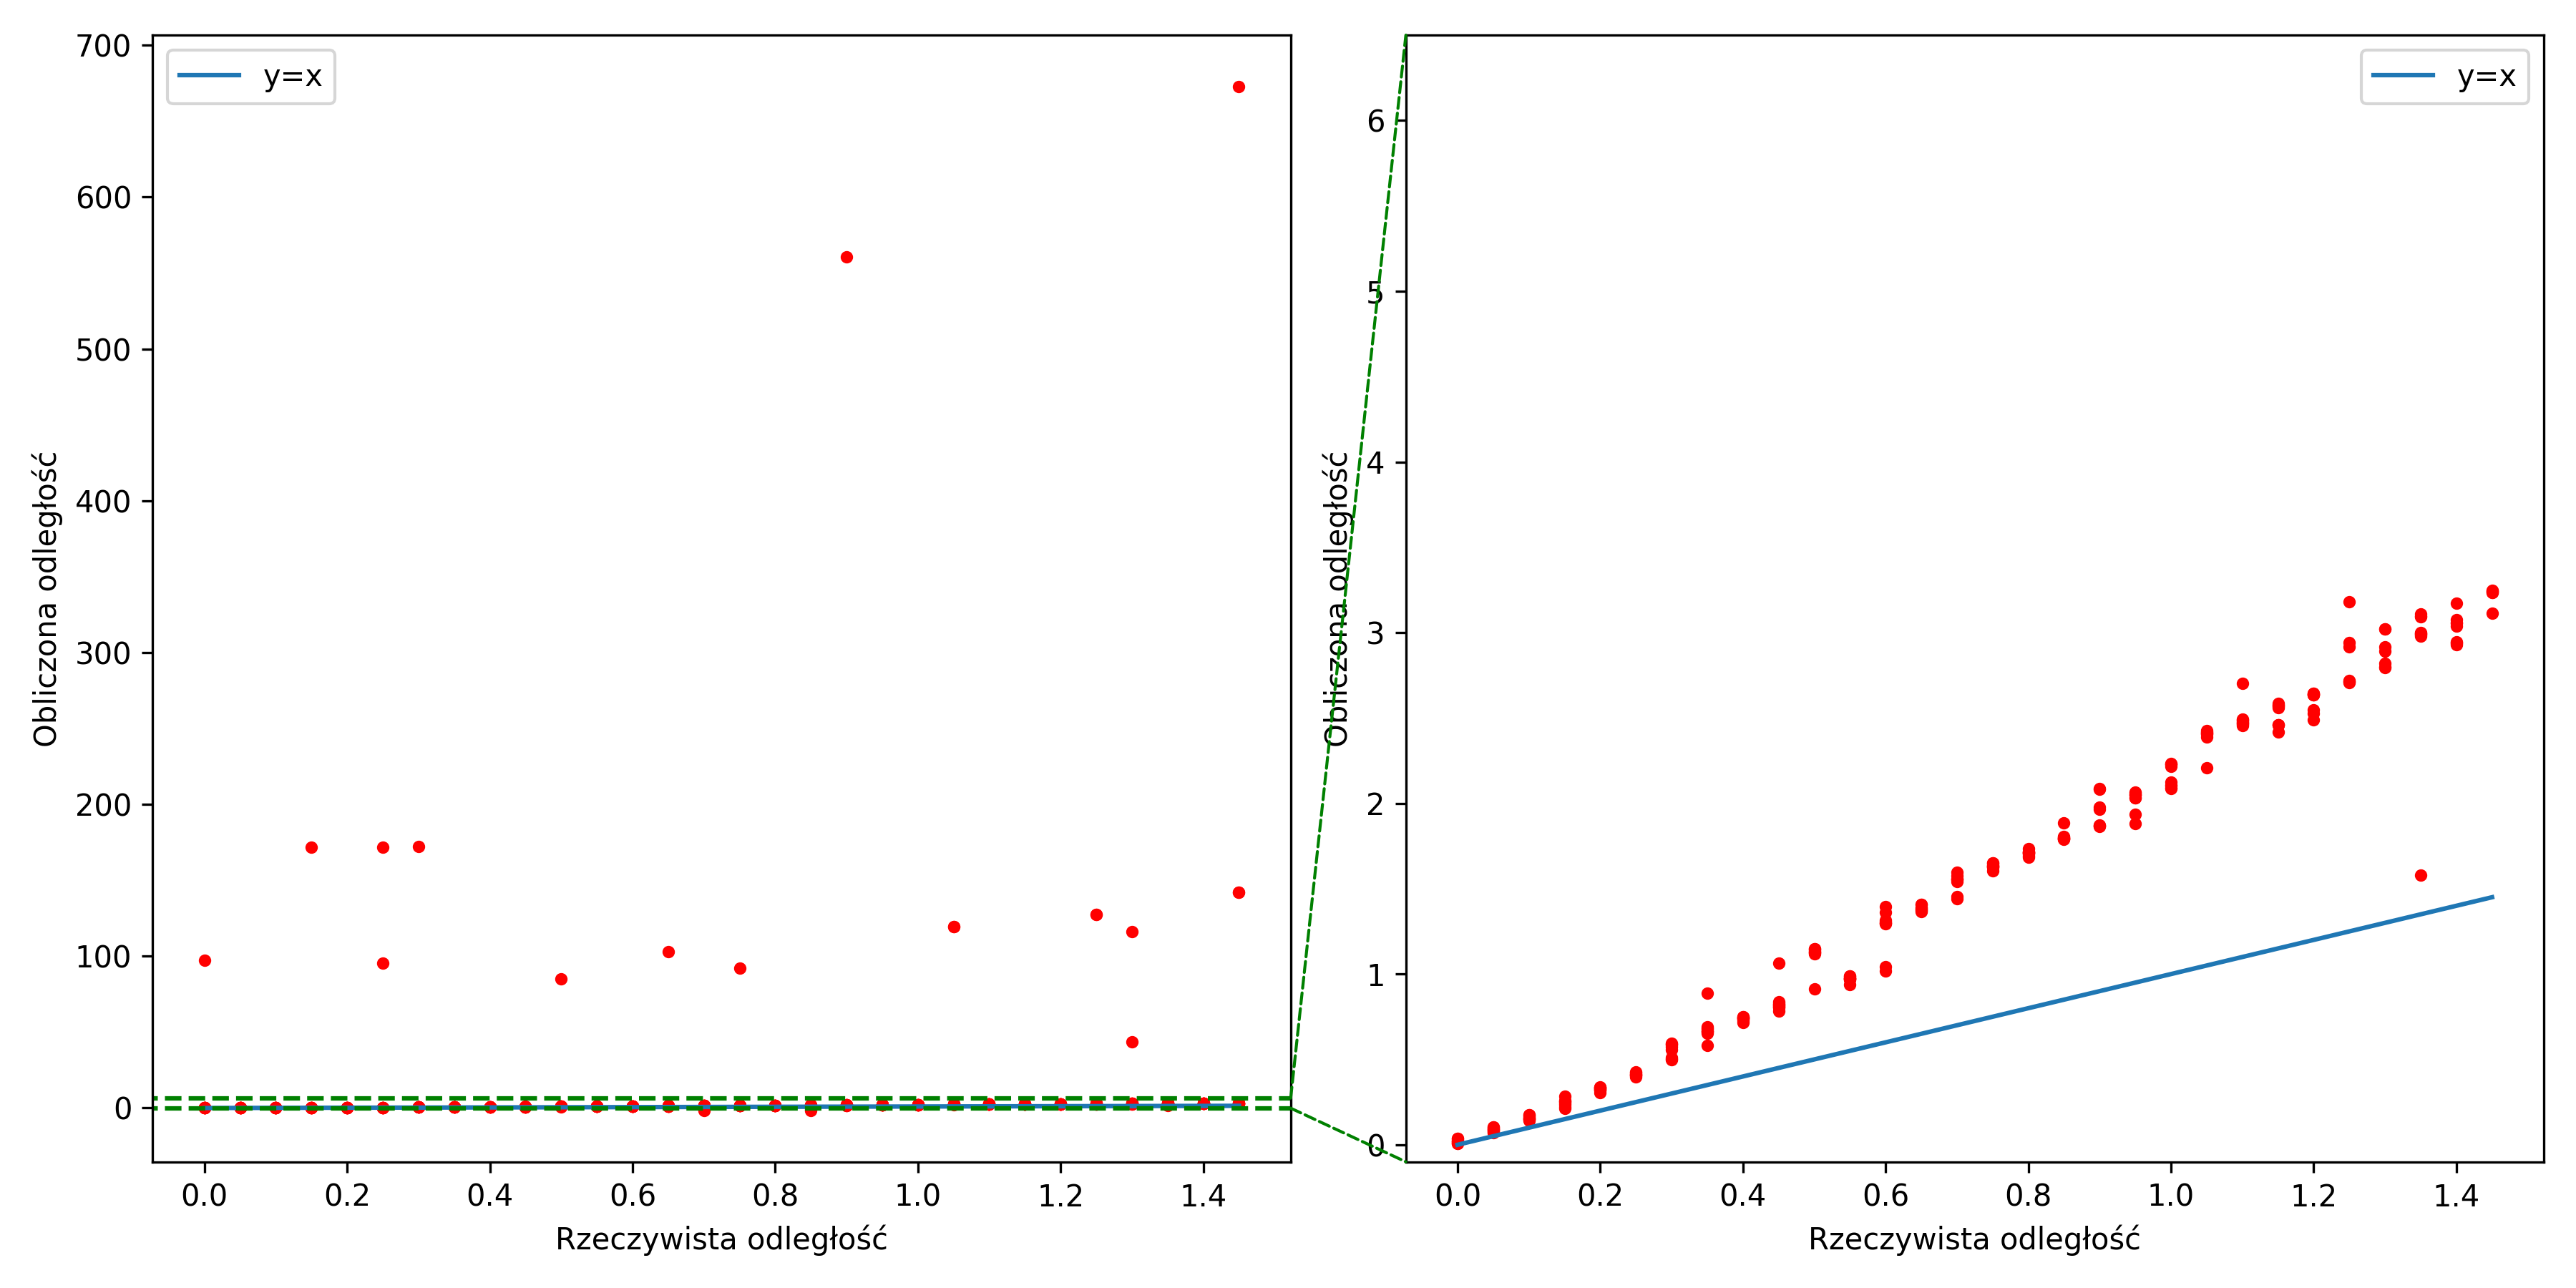
\includegraphics[width=.49\textwidth]{pics/mic_sync_dist/dists_long_0.png}
    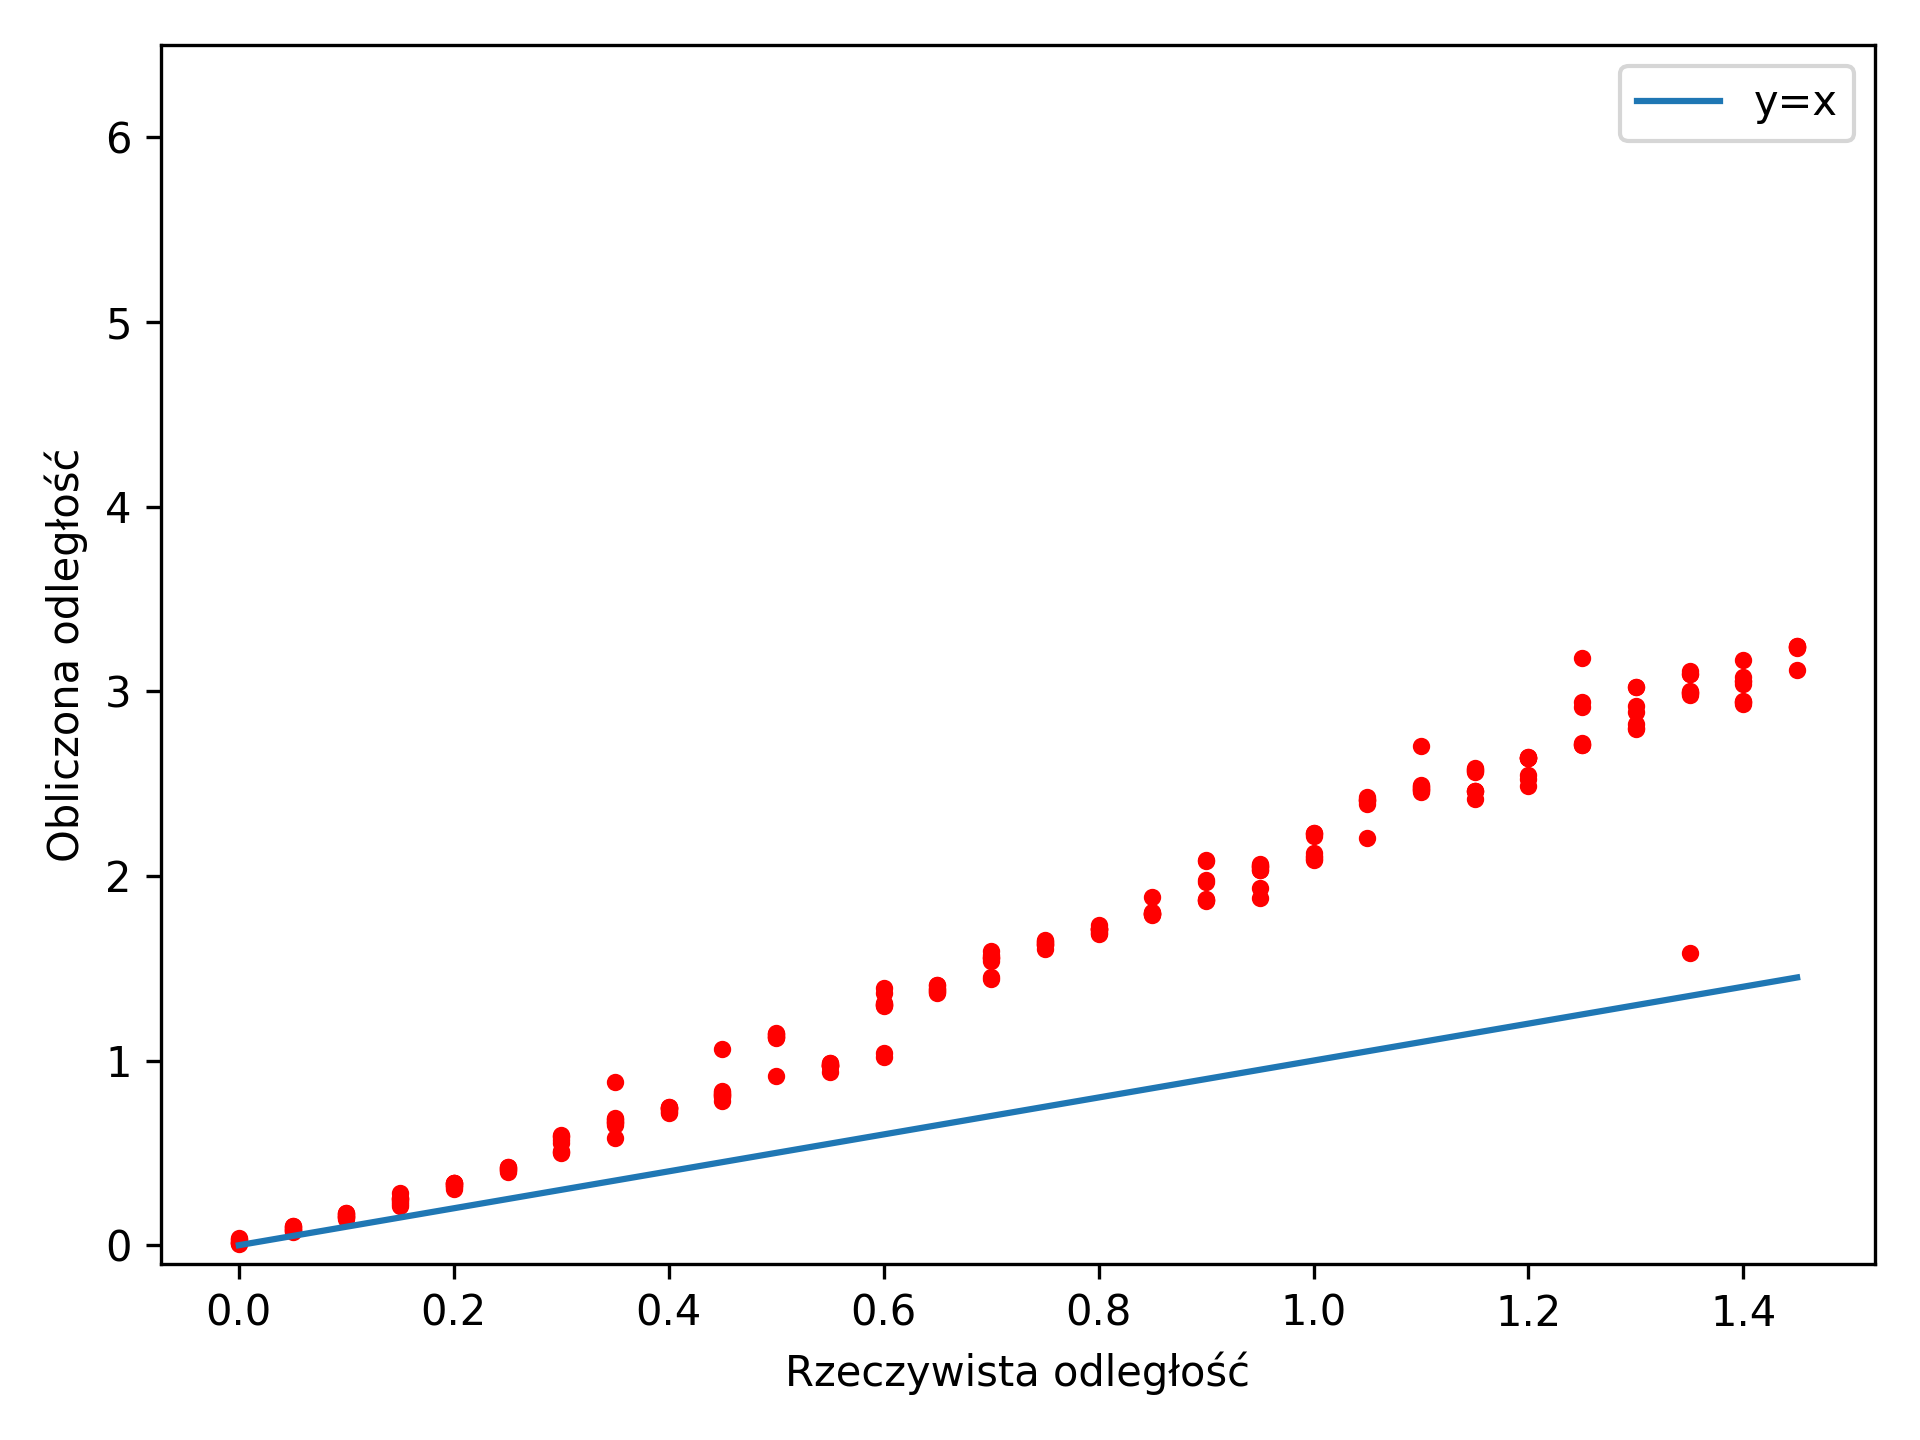
\includegraphics[width=.49\textwidth]{pics/mic_sync_dist/dists_close_long_0.png}
\caption{Pomiar obliczanych odległości 1.}
\label{pic:slope_test_0}
\end{figure}

\begin{figure}[h]
\centering
    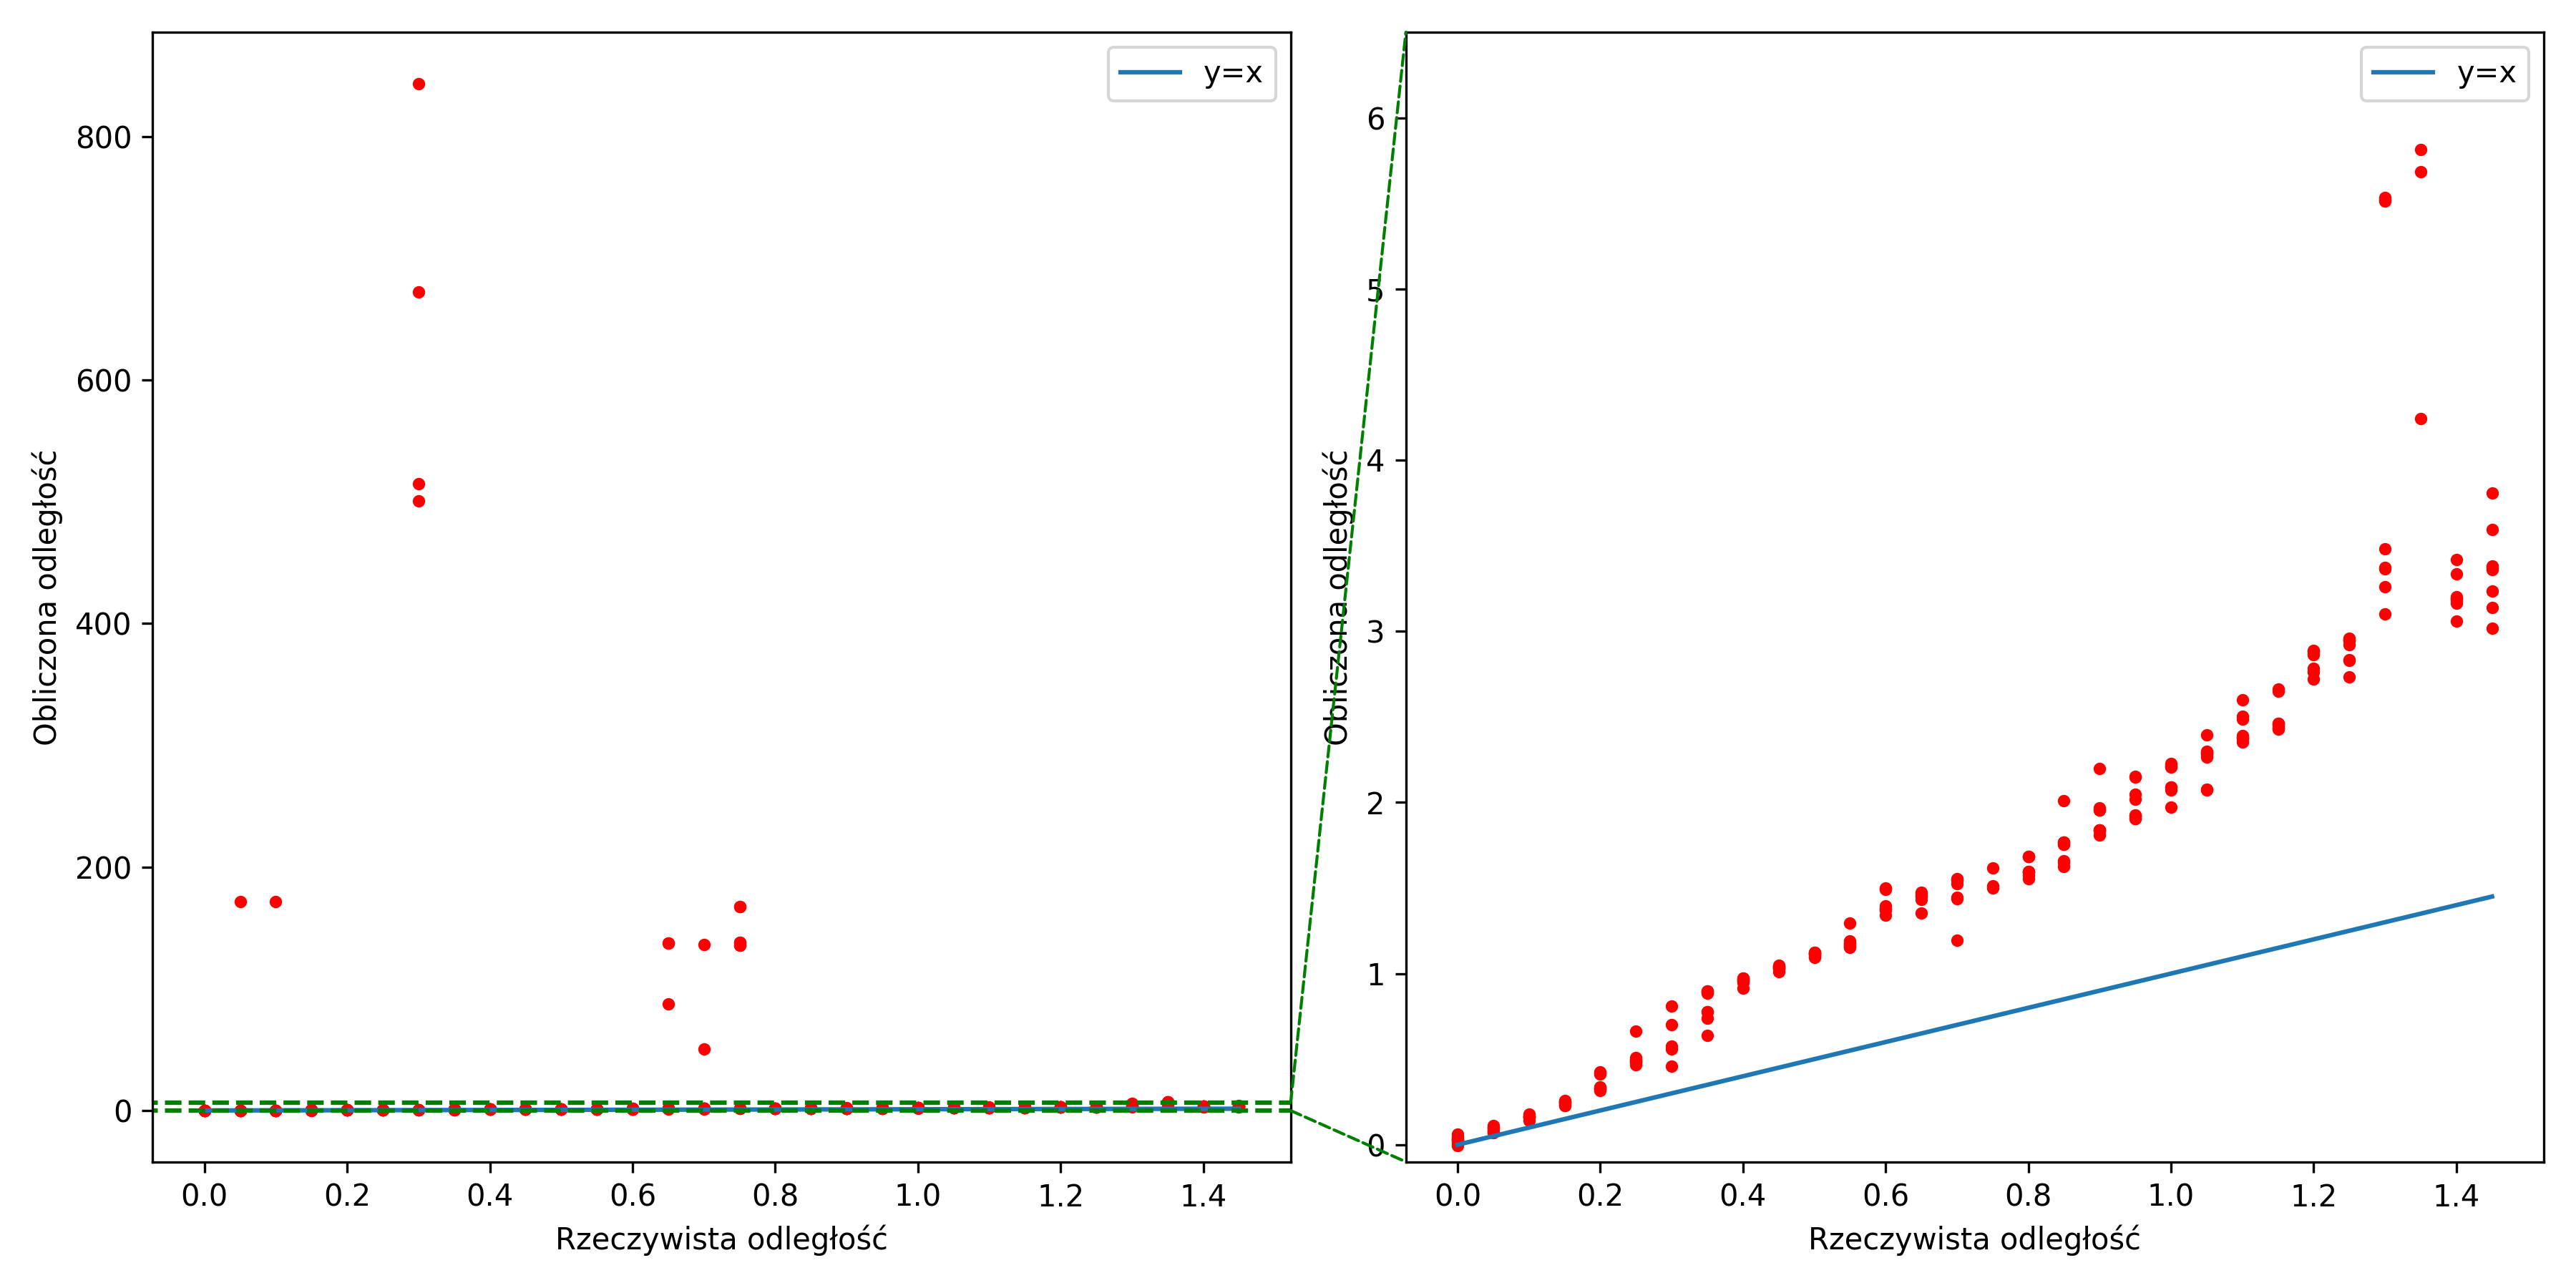
\includegraphics[width=.49\textwidth]{pics/mic_sync_dist/dists_long_1.png}
    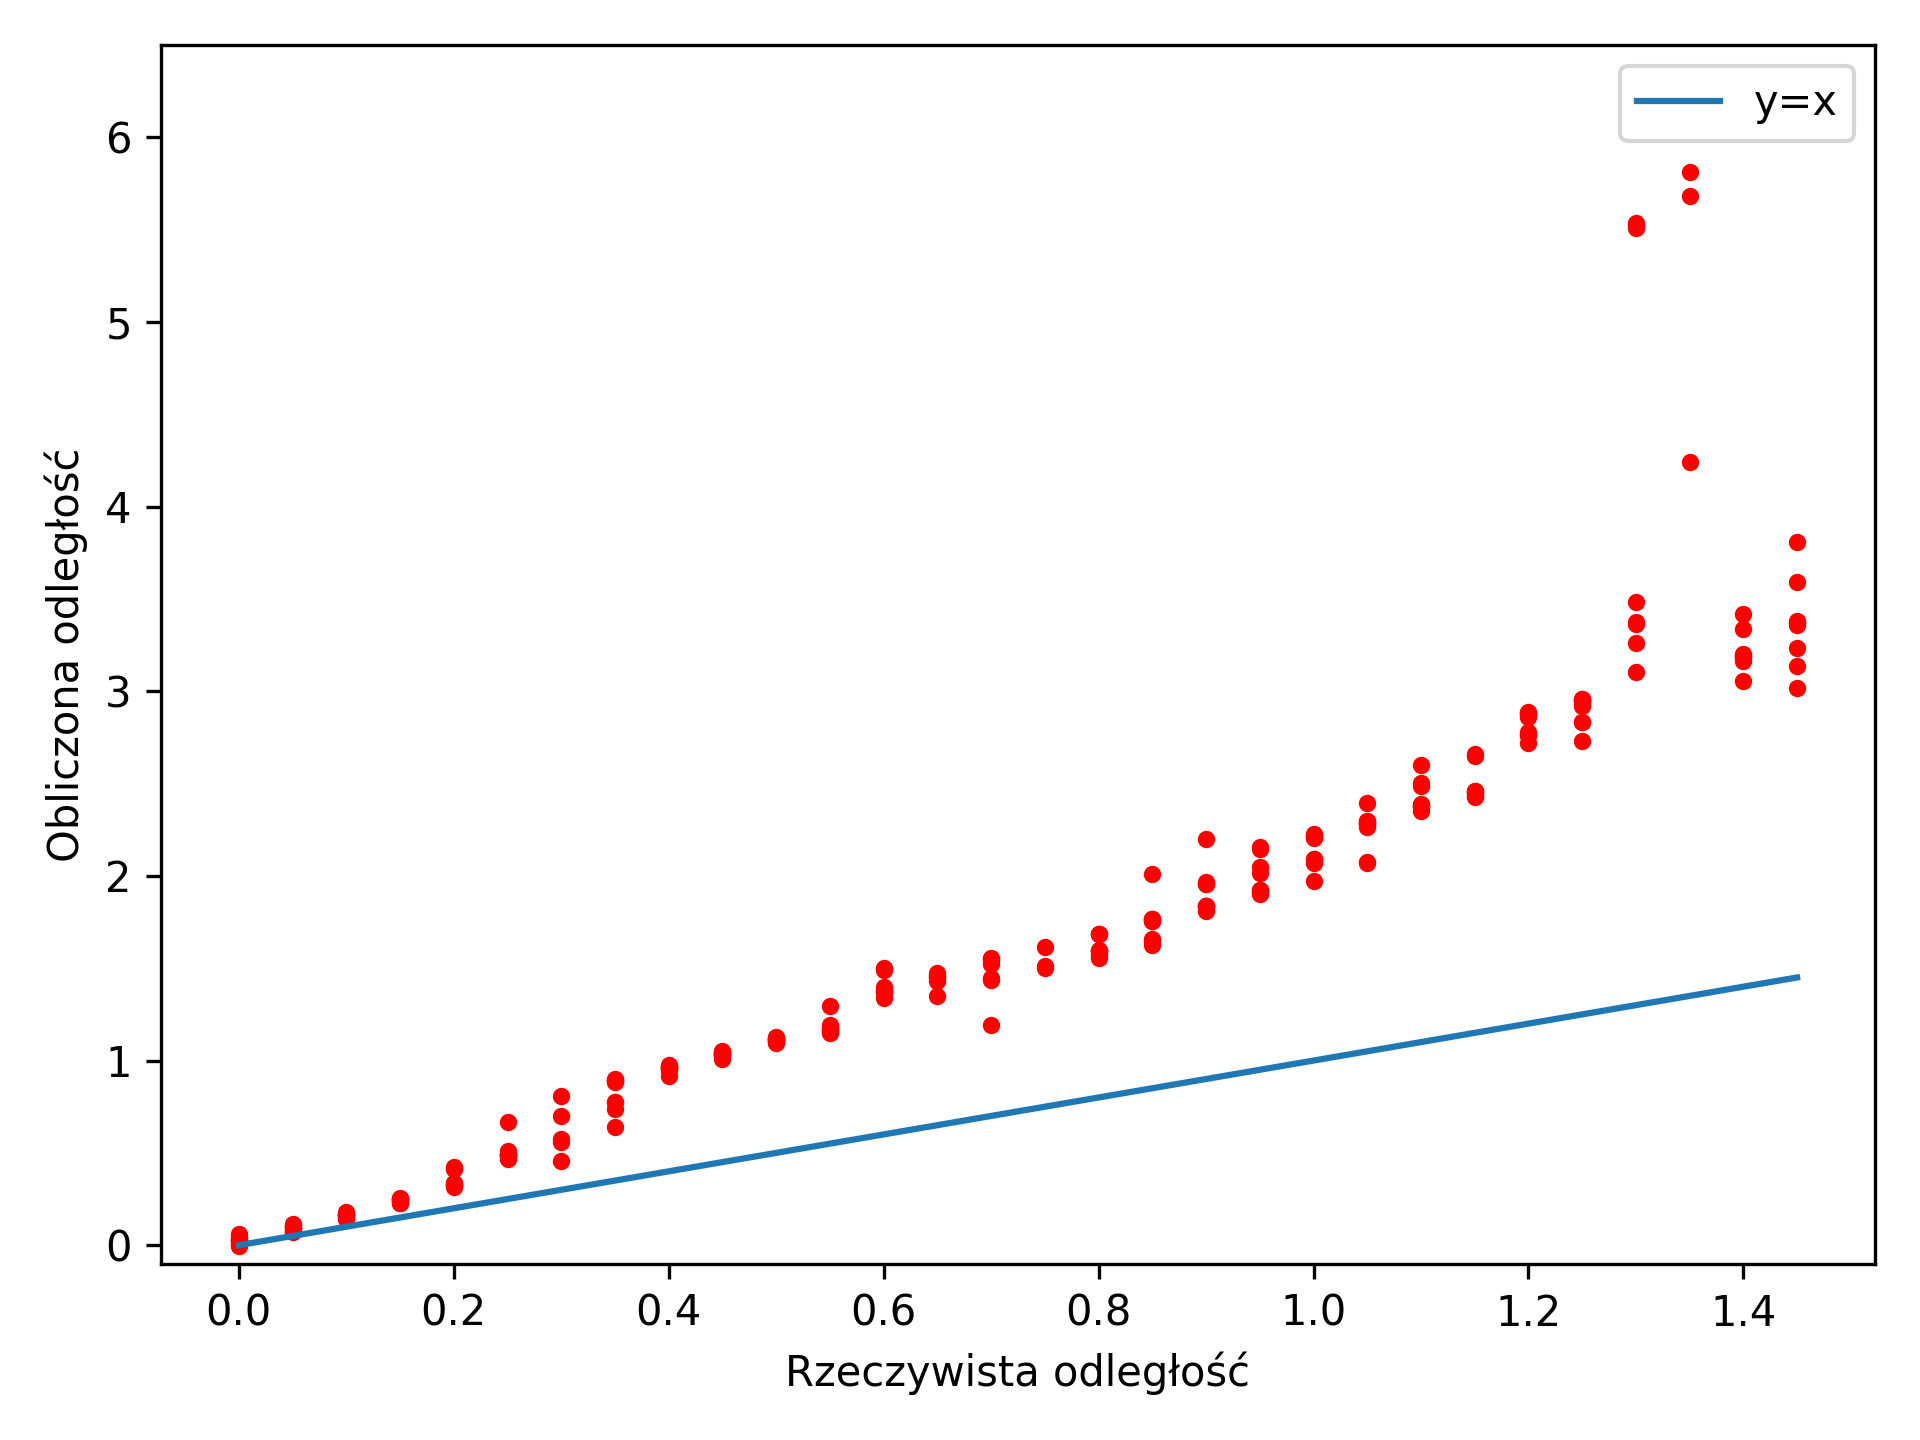
\includegraphics[width=.49\textwidth]{pics/mic_sync_dist/dists_close_long_1.png}
\caption{Pomiar obliczanych odległości 2.}
\label{pic:slope_test_1}
\end{figure}

\begin{figure}[h]
\centering
    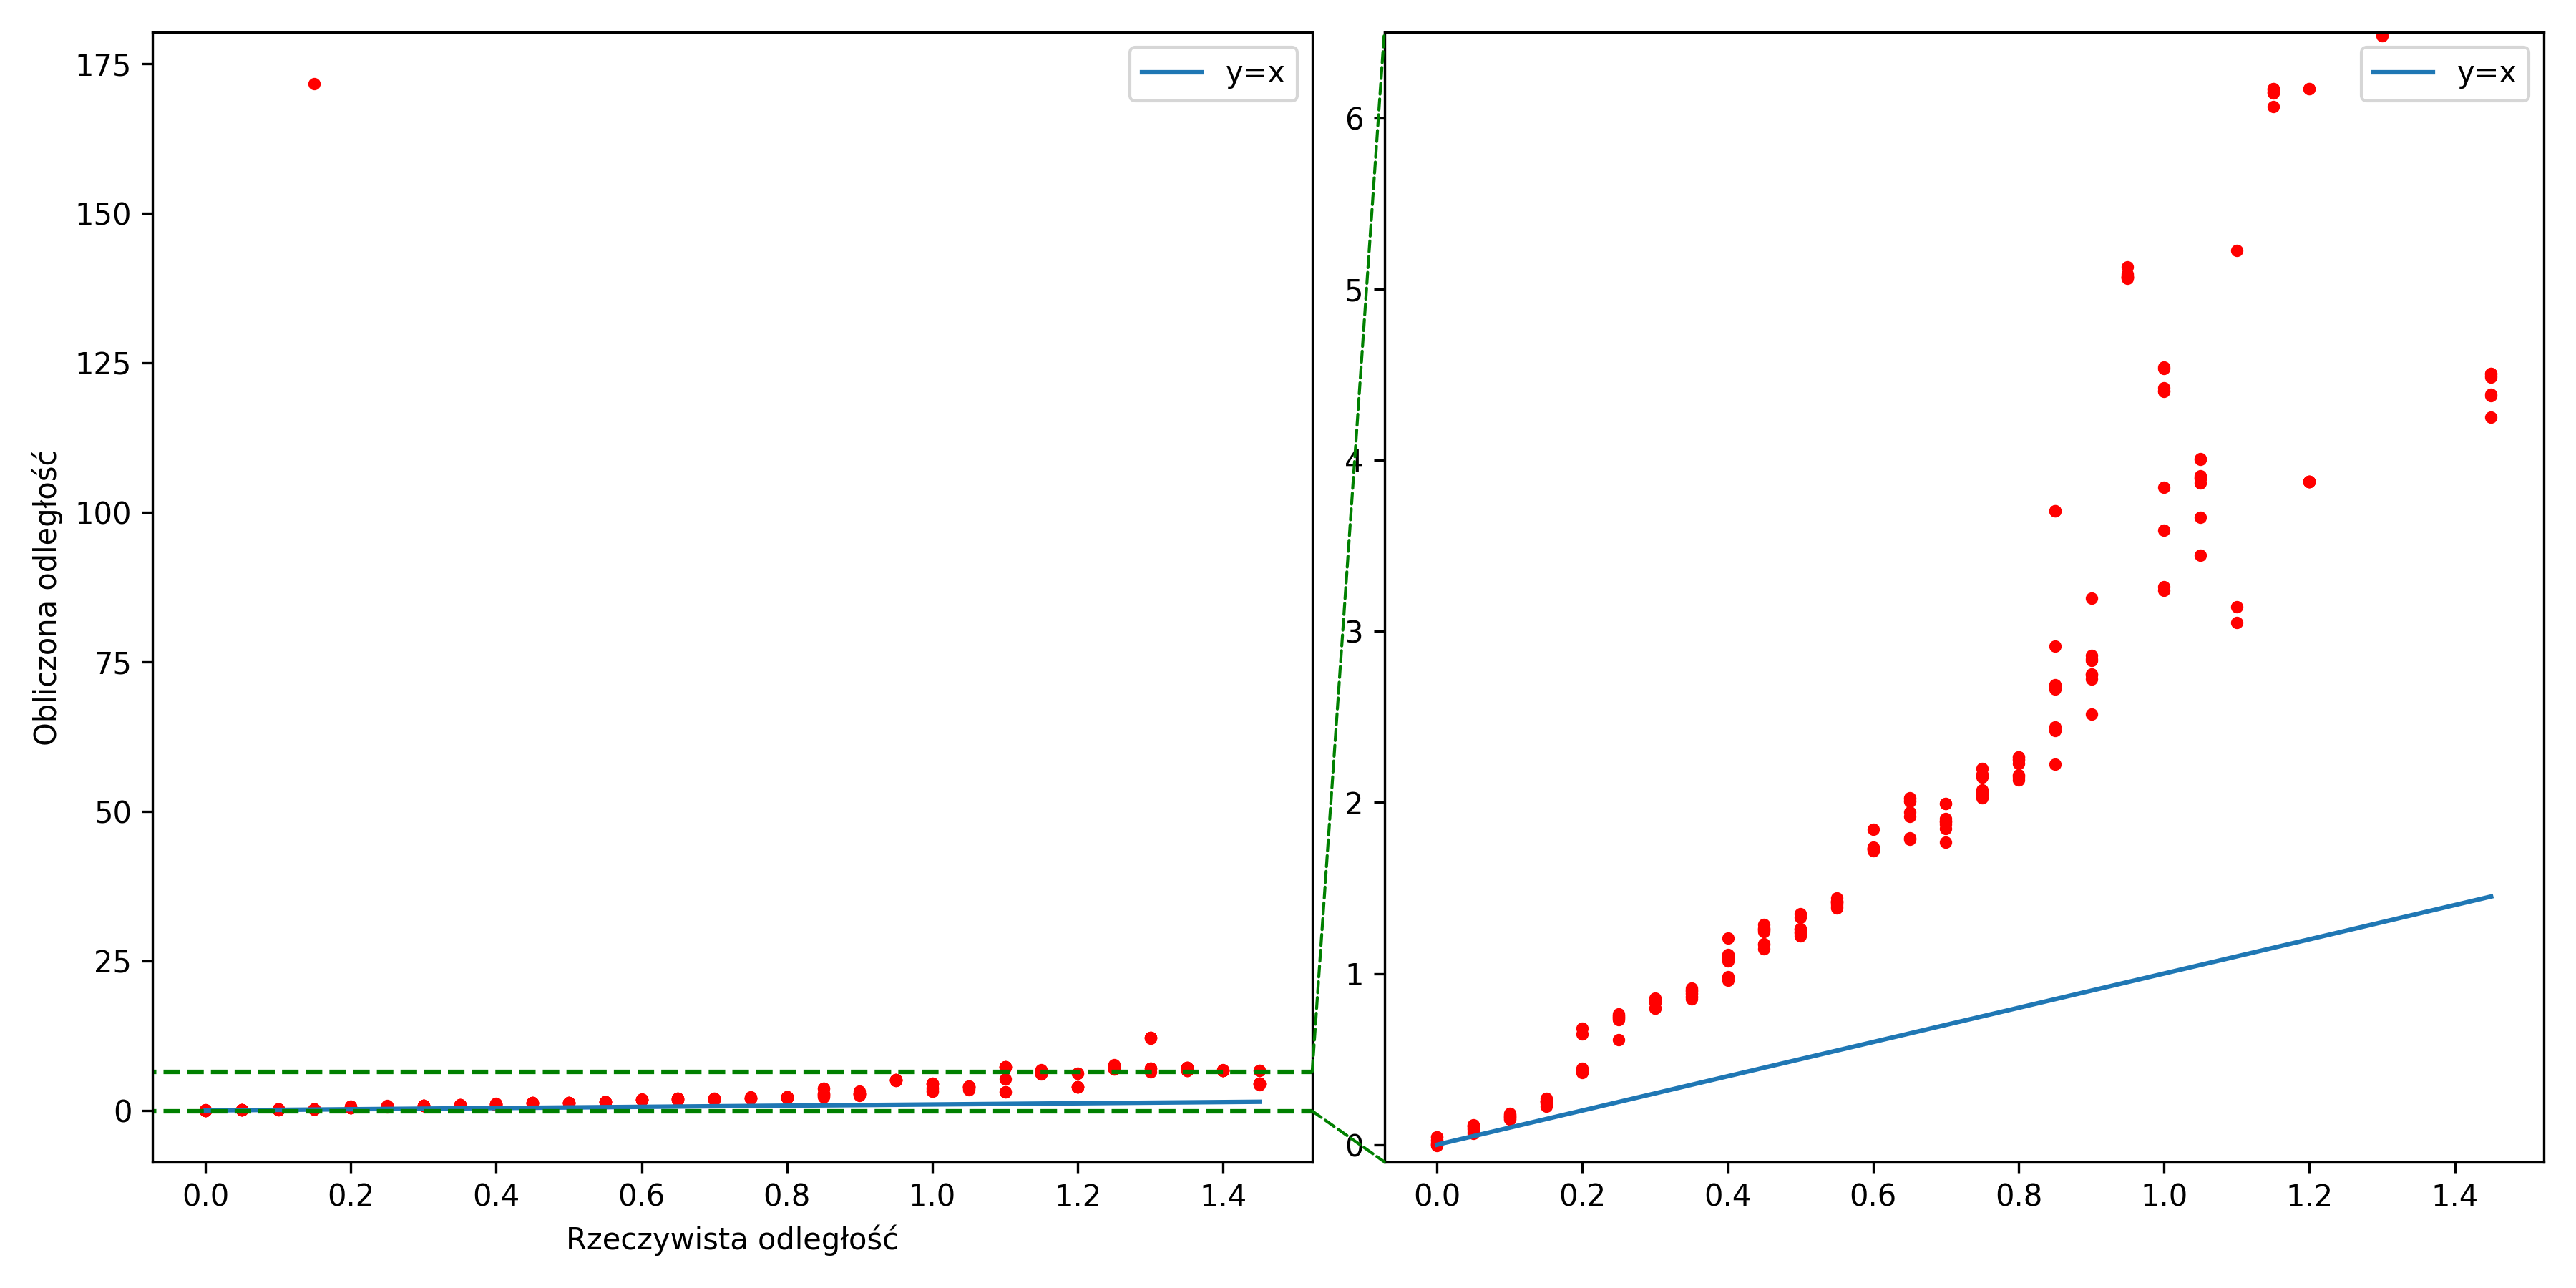
\includegraphics[width=.49\textwidth]{pics/mic_sync_dist/dists_long_2.png}
    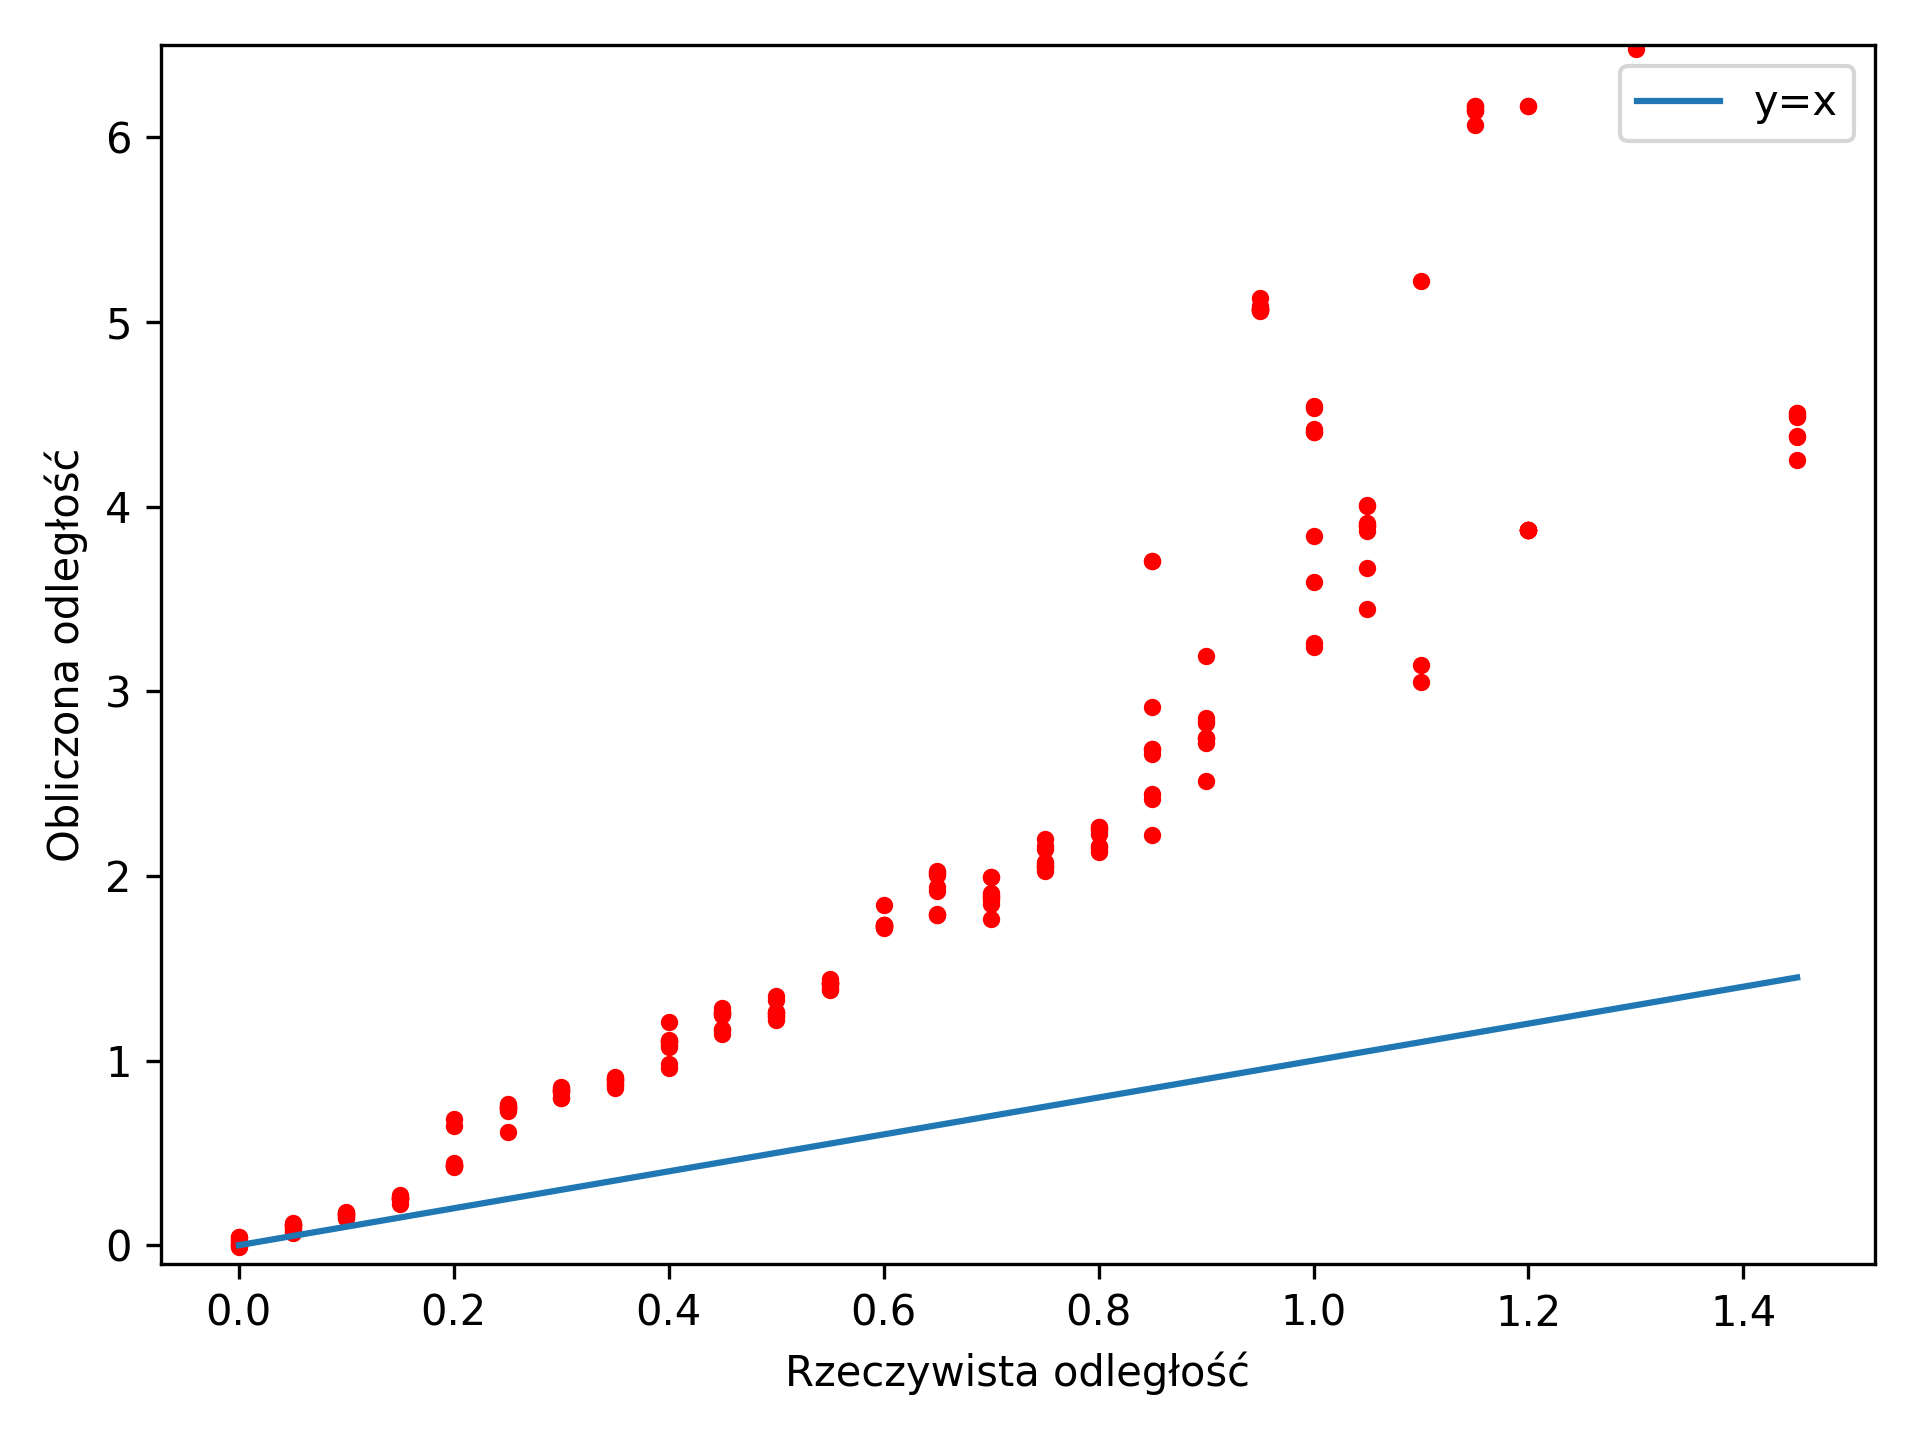
\includegraphics[width=.49\textwidth]{pics/mic_sync_dist/dists_close_long_2.png}
\caption{Pomiar obliczanych odległości 3.}
\label{pic:slope_test_2}
\end{figure}

\begin{figure}[h]
\centering
    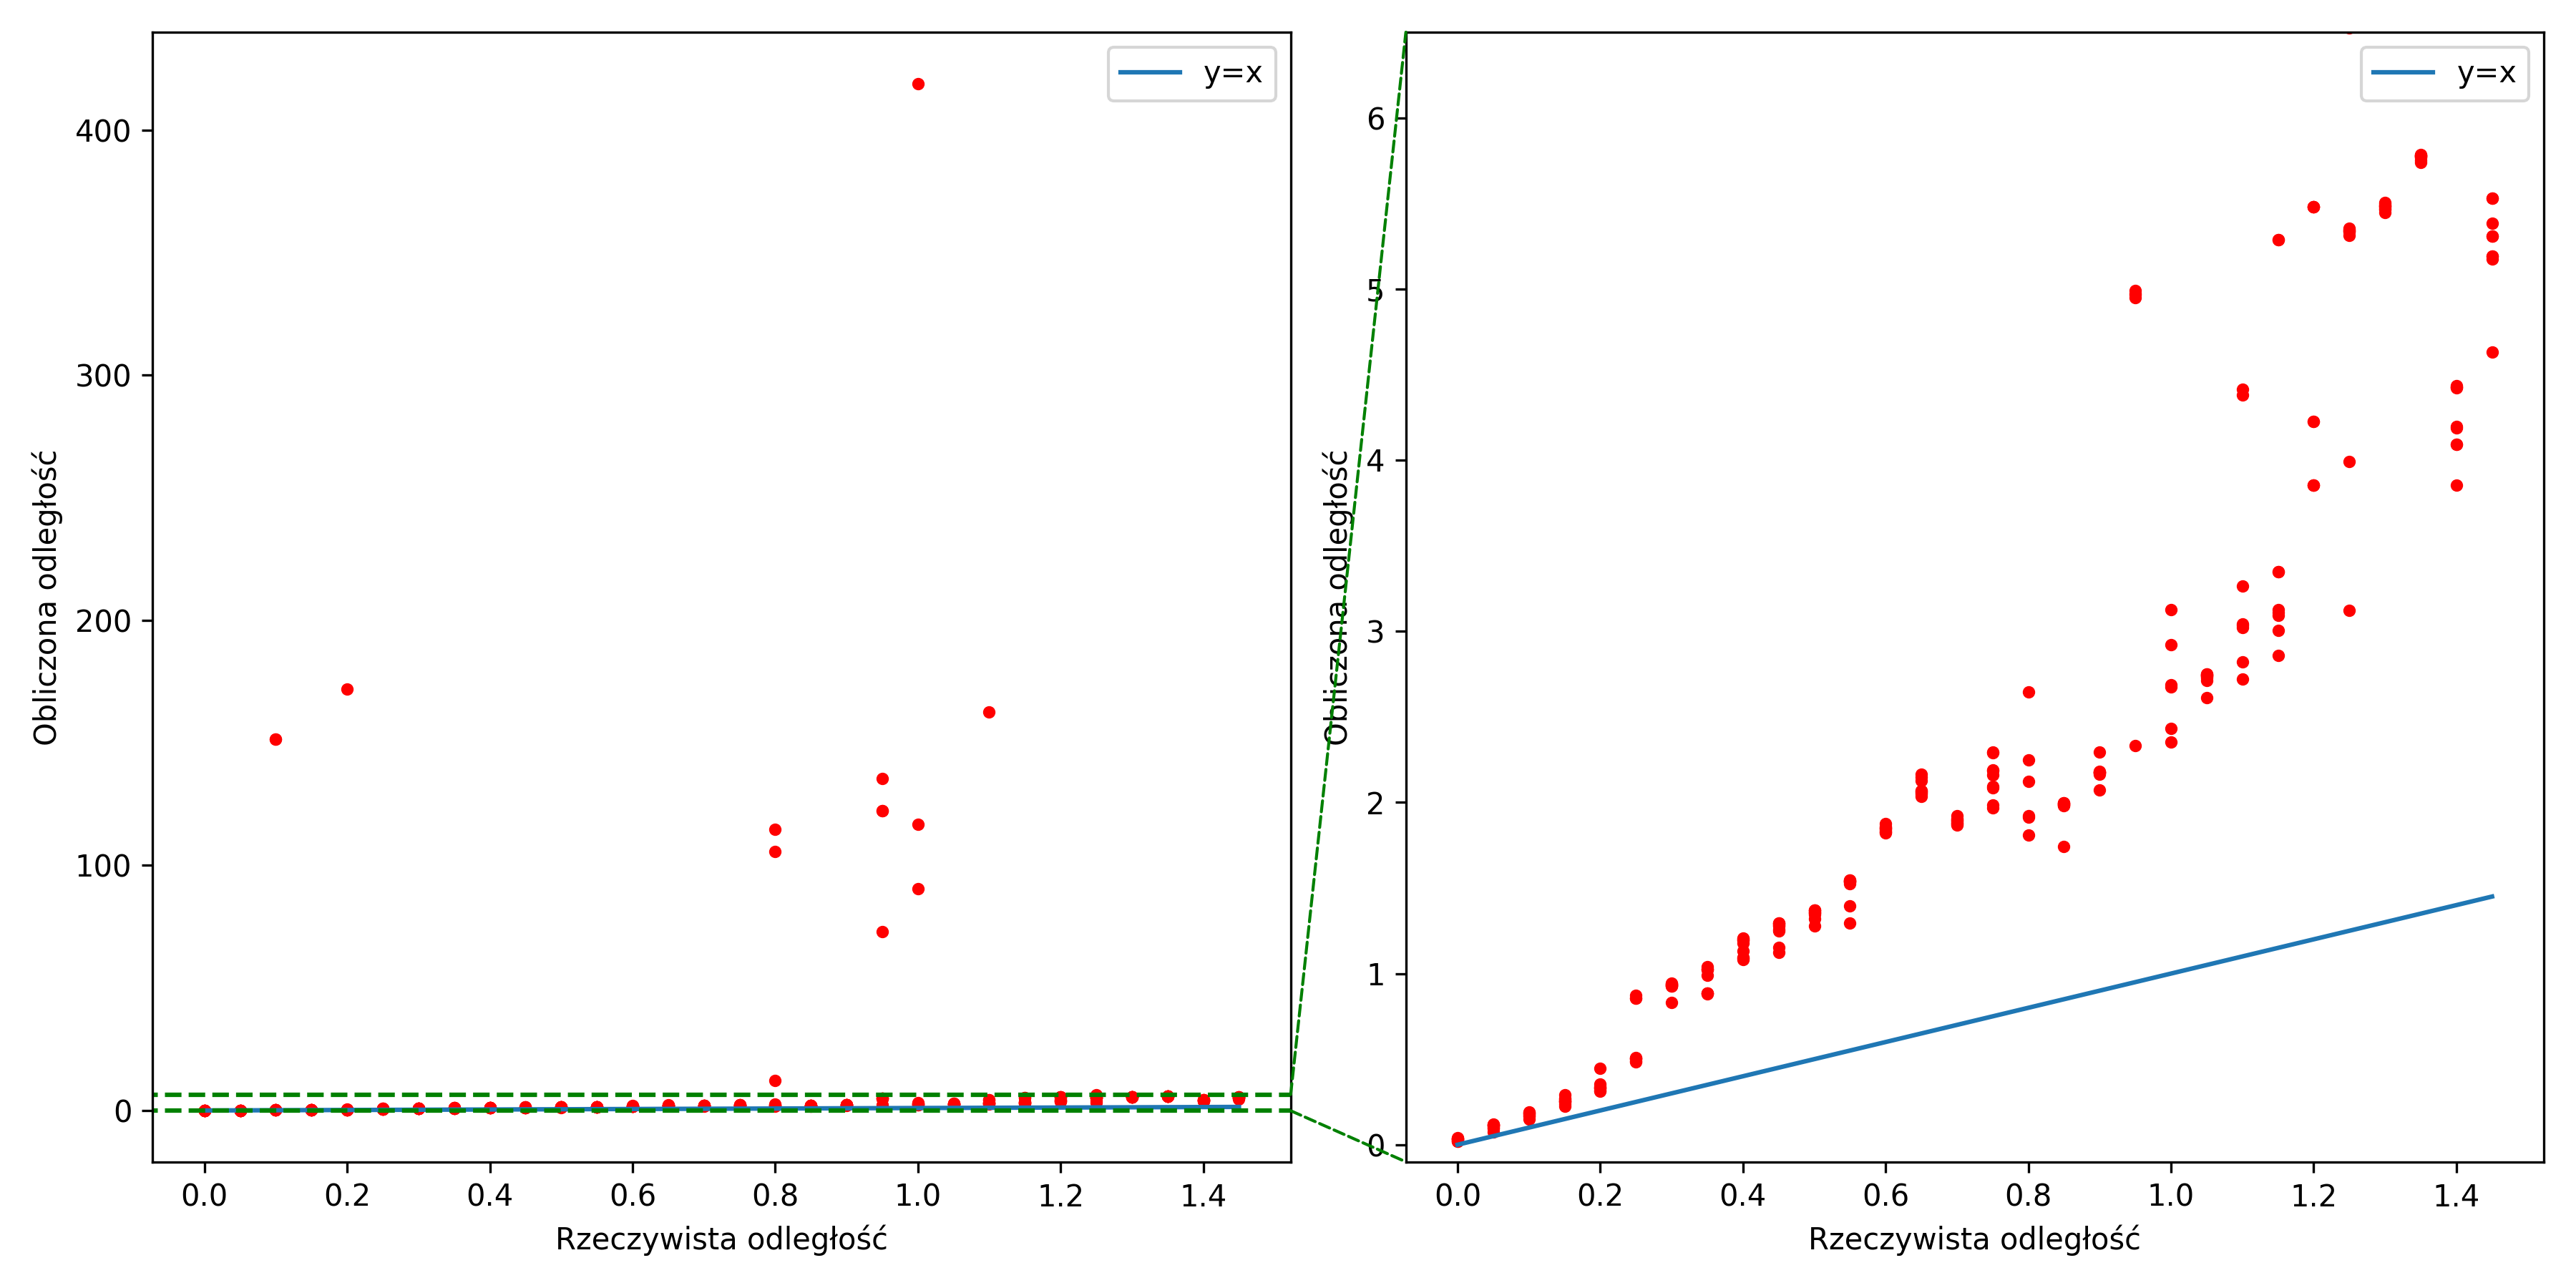
\includegraphics[width=.49\textwidth]{pics/mic_sync_dist/dists_long_3.png}
    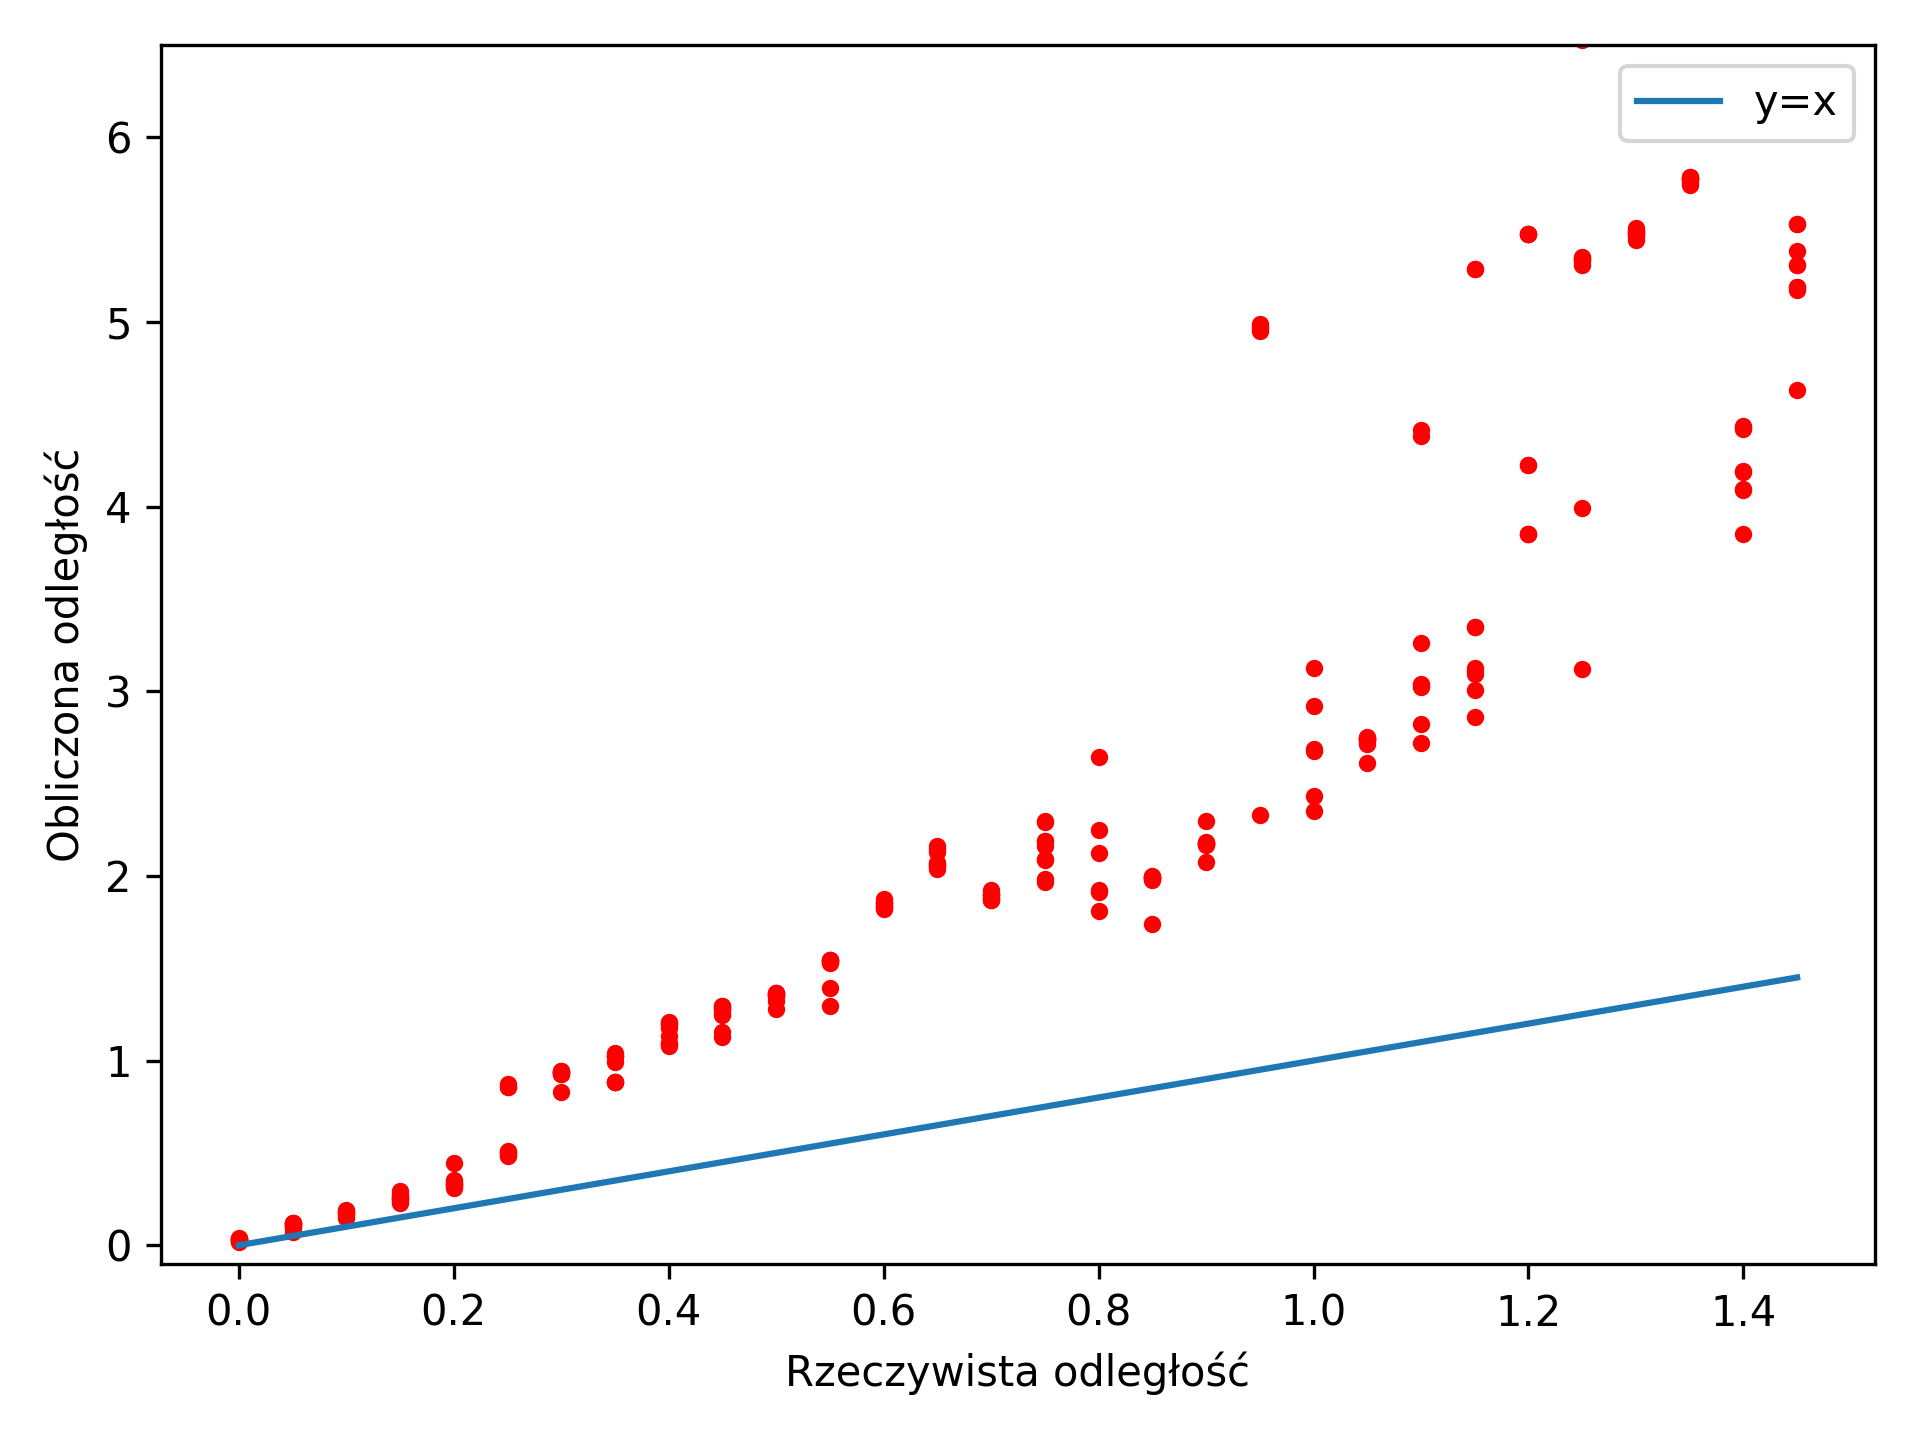
\includegraphics[width=.49\textwidth]{pics/mic_sync_dist/dists_close_long_3.png}
\caption{Pomiar obliczanych odległości 4.}
\label{pic:slope_test_3}
\end{figure}

Aby lepiej odczytać informacje z wykresu uśrednijmy pomiary dla każdej z badanych odległości i dodajmy do nich funkcje liniowe o współczynniku otrzymanym przy pomocy regresji liniowej z tychże uśrednionych punktów.

\begin{figure}[h]
\centering
    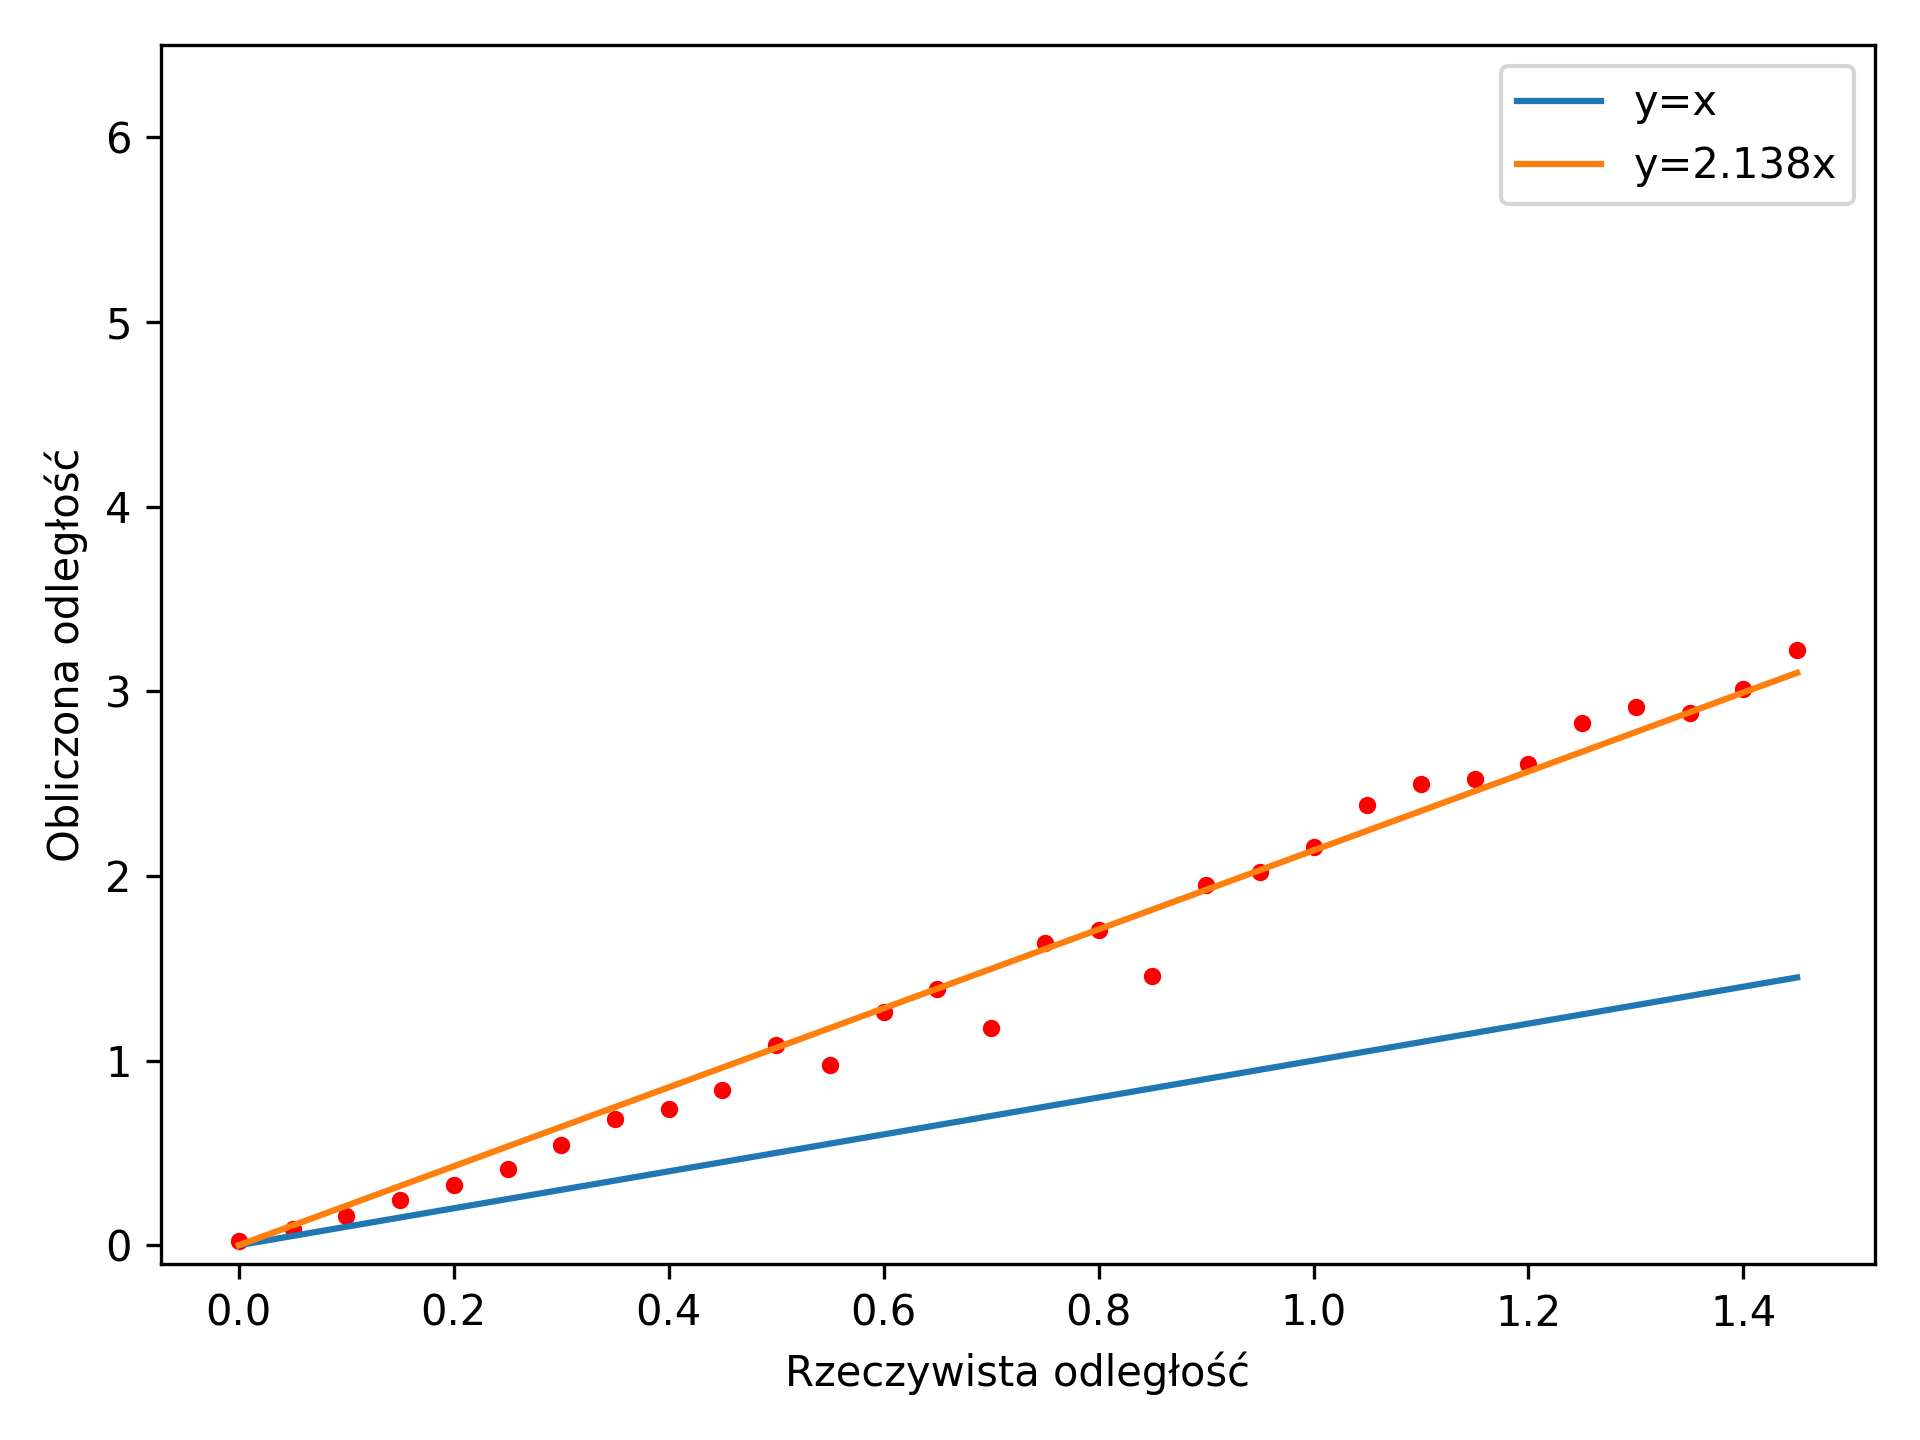
\includegraphics[width=.49\textwidth]{pics/mic_sync_dist/dists_close_long_0_mean.png}
    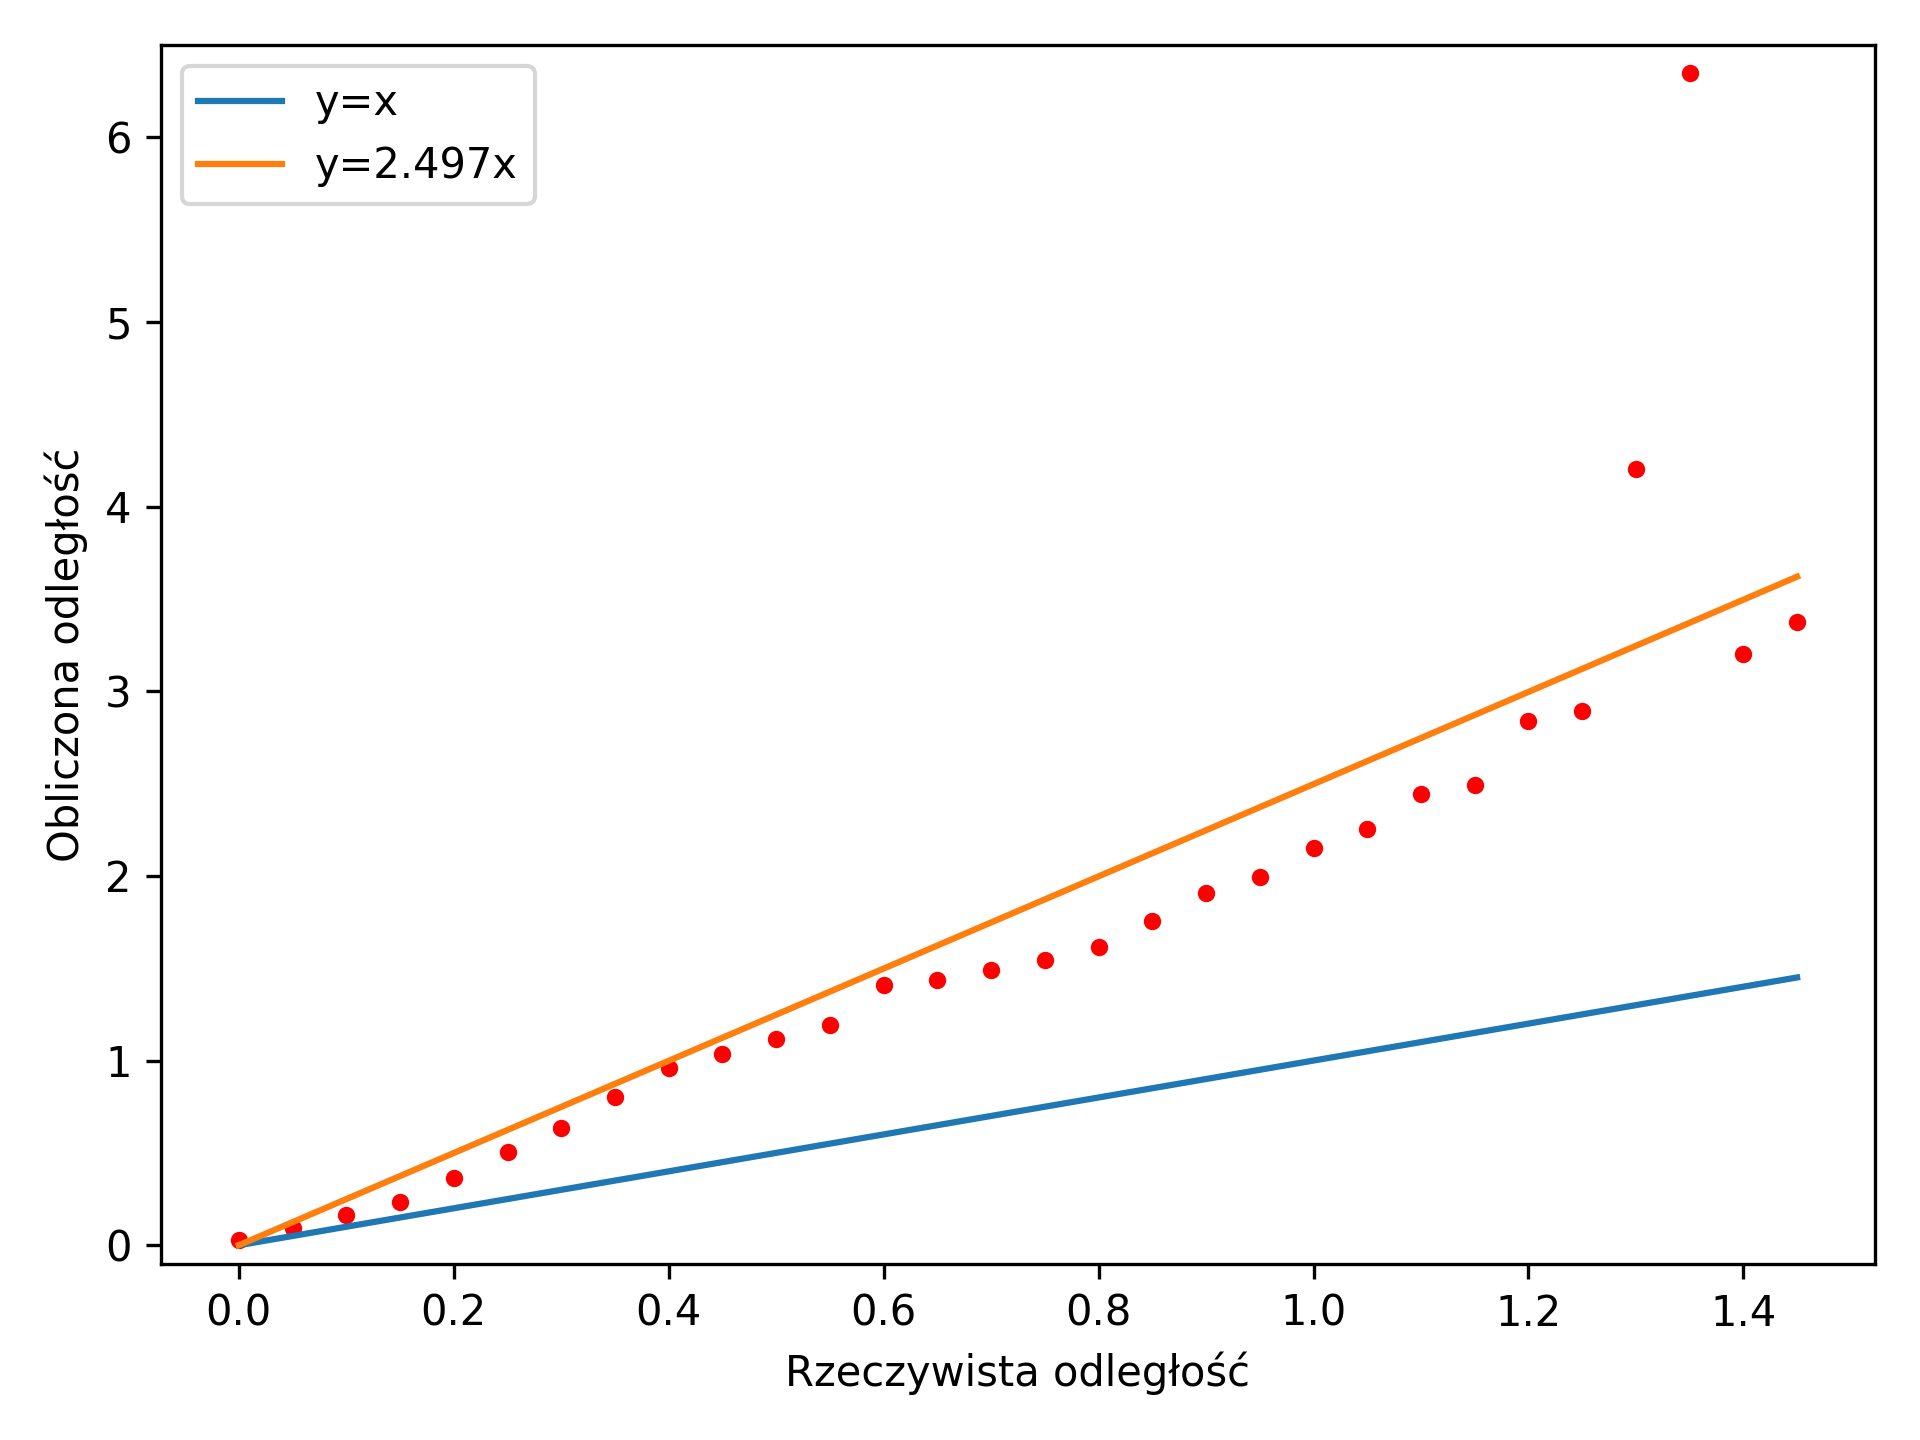
\includegraphics[width=.49\textwidth]{pics/mic_sync_dist/dists_close_long_1_mean.png}
    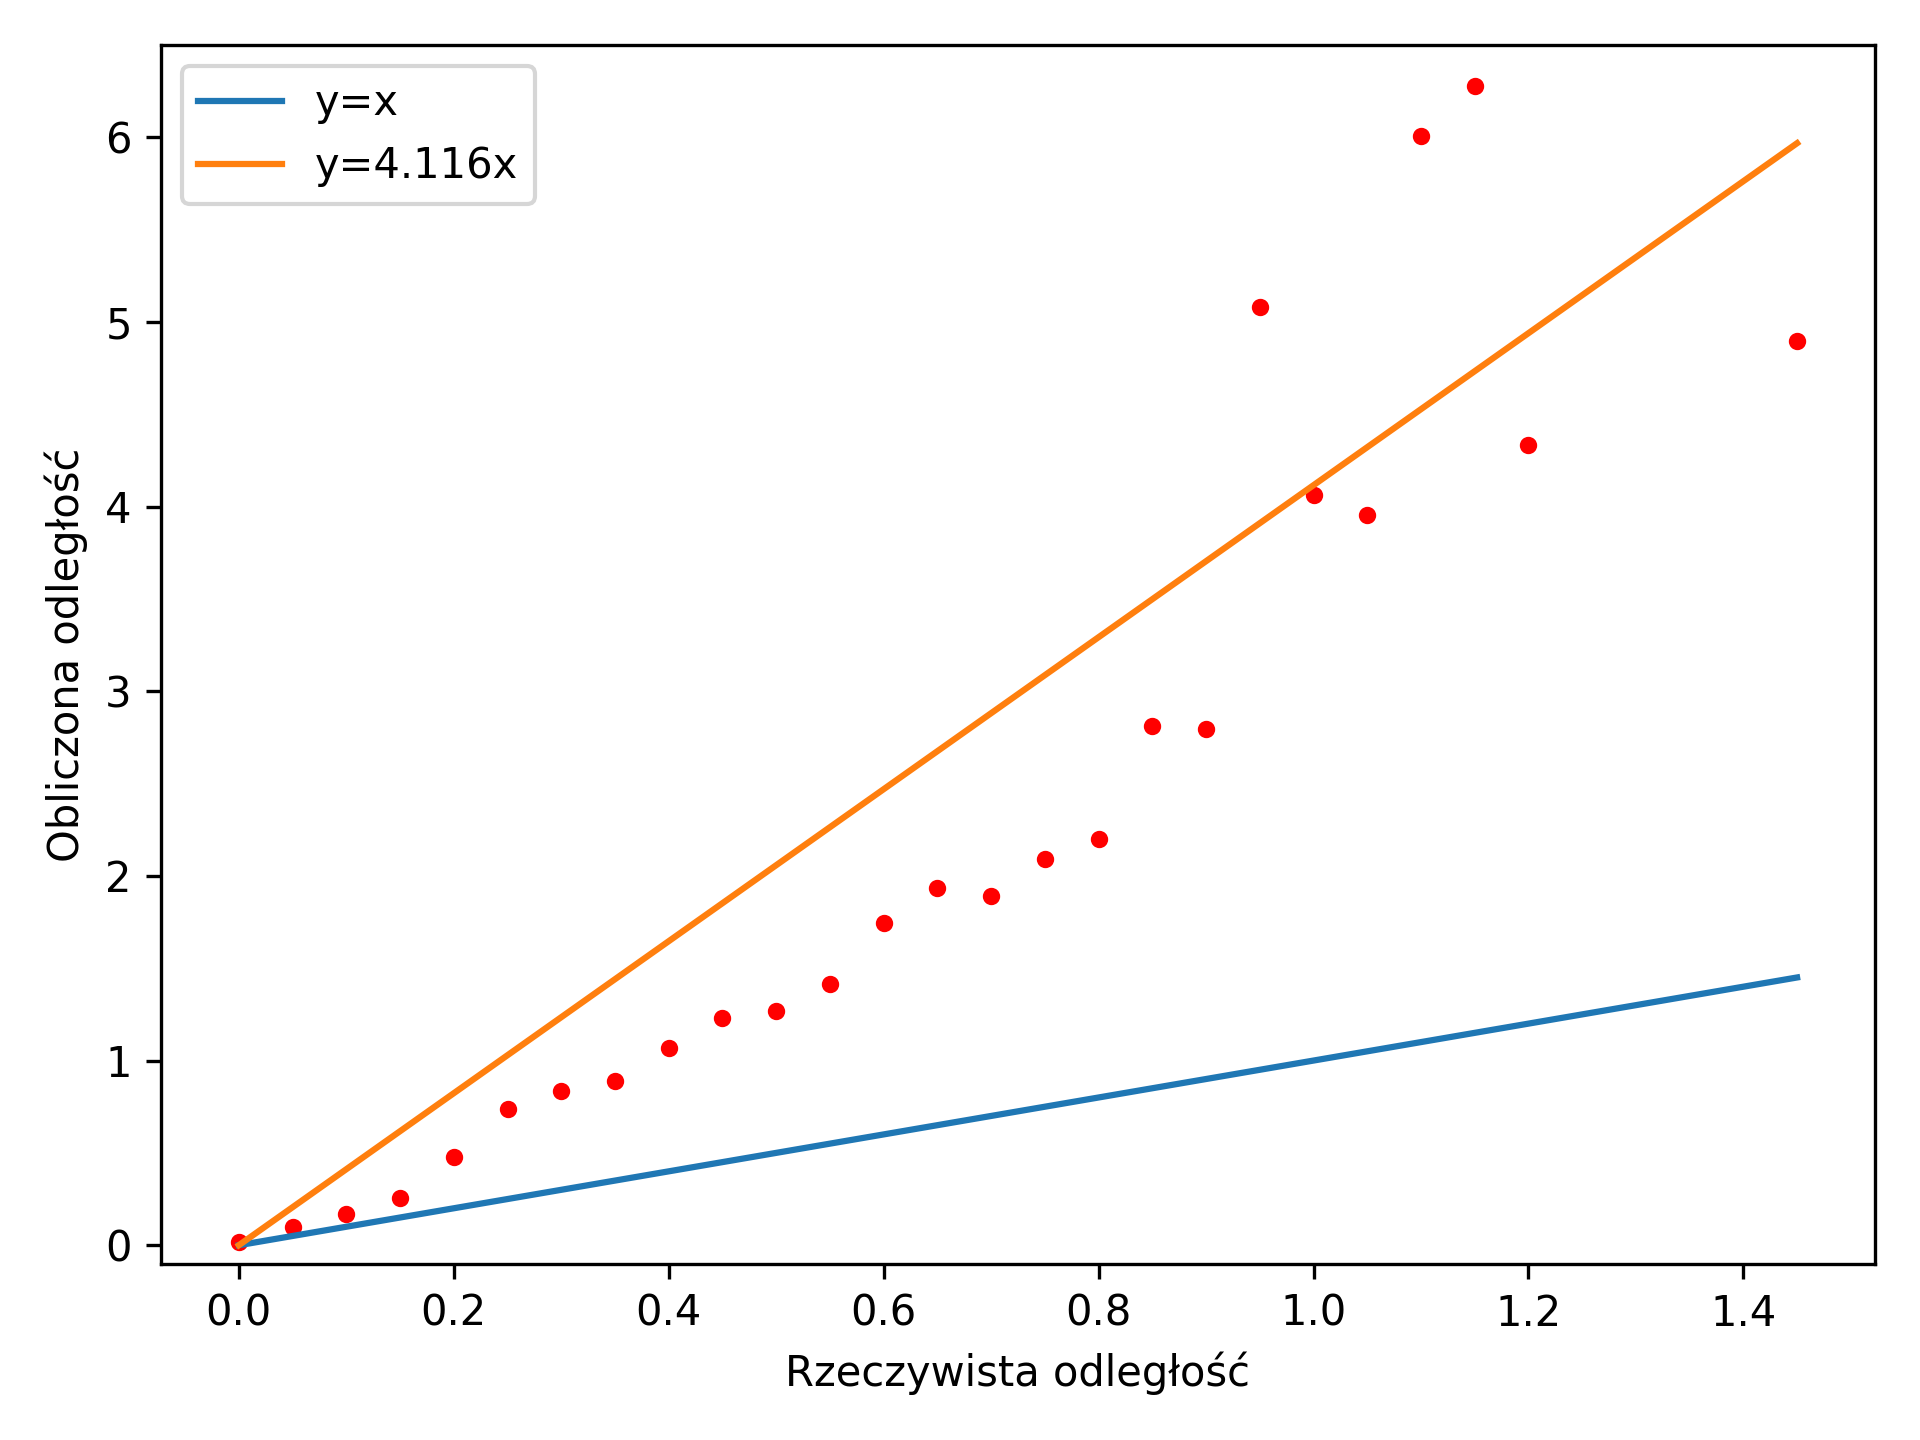
\includegraphics[width=.49\textwidth]{pics/mic_sync_dist/dists_close_long_2_mean.png}
    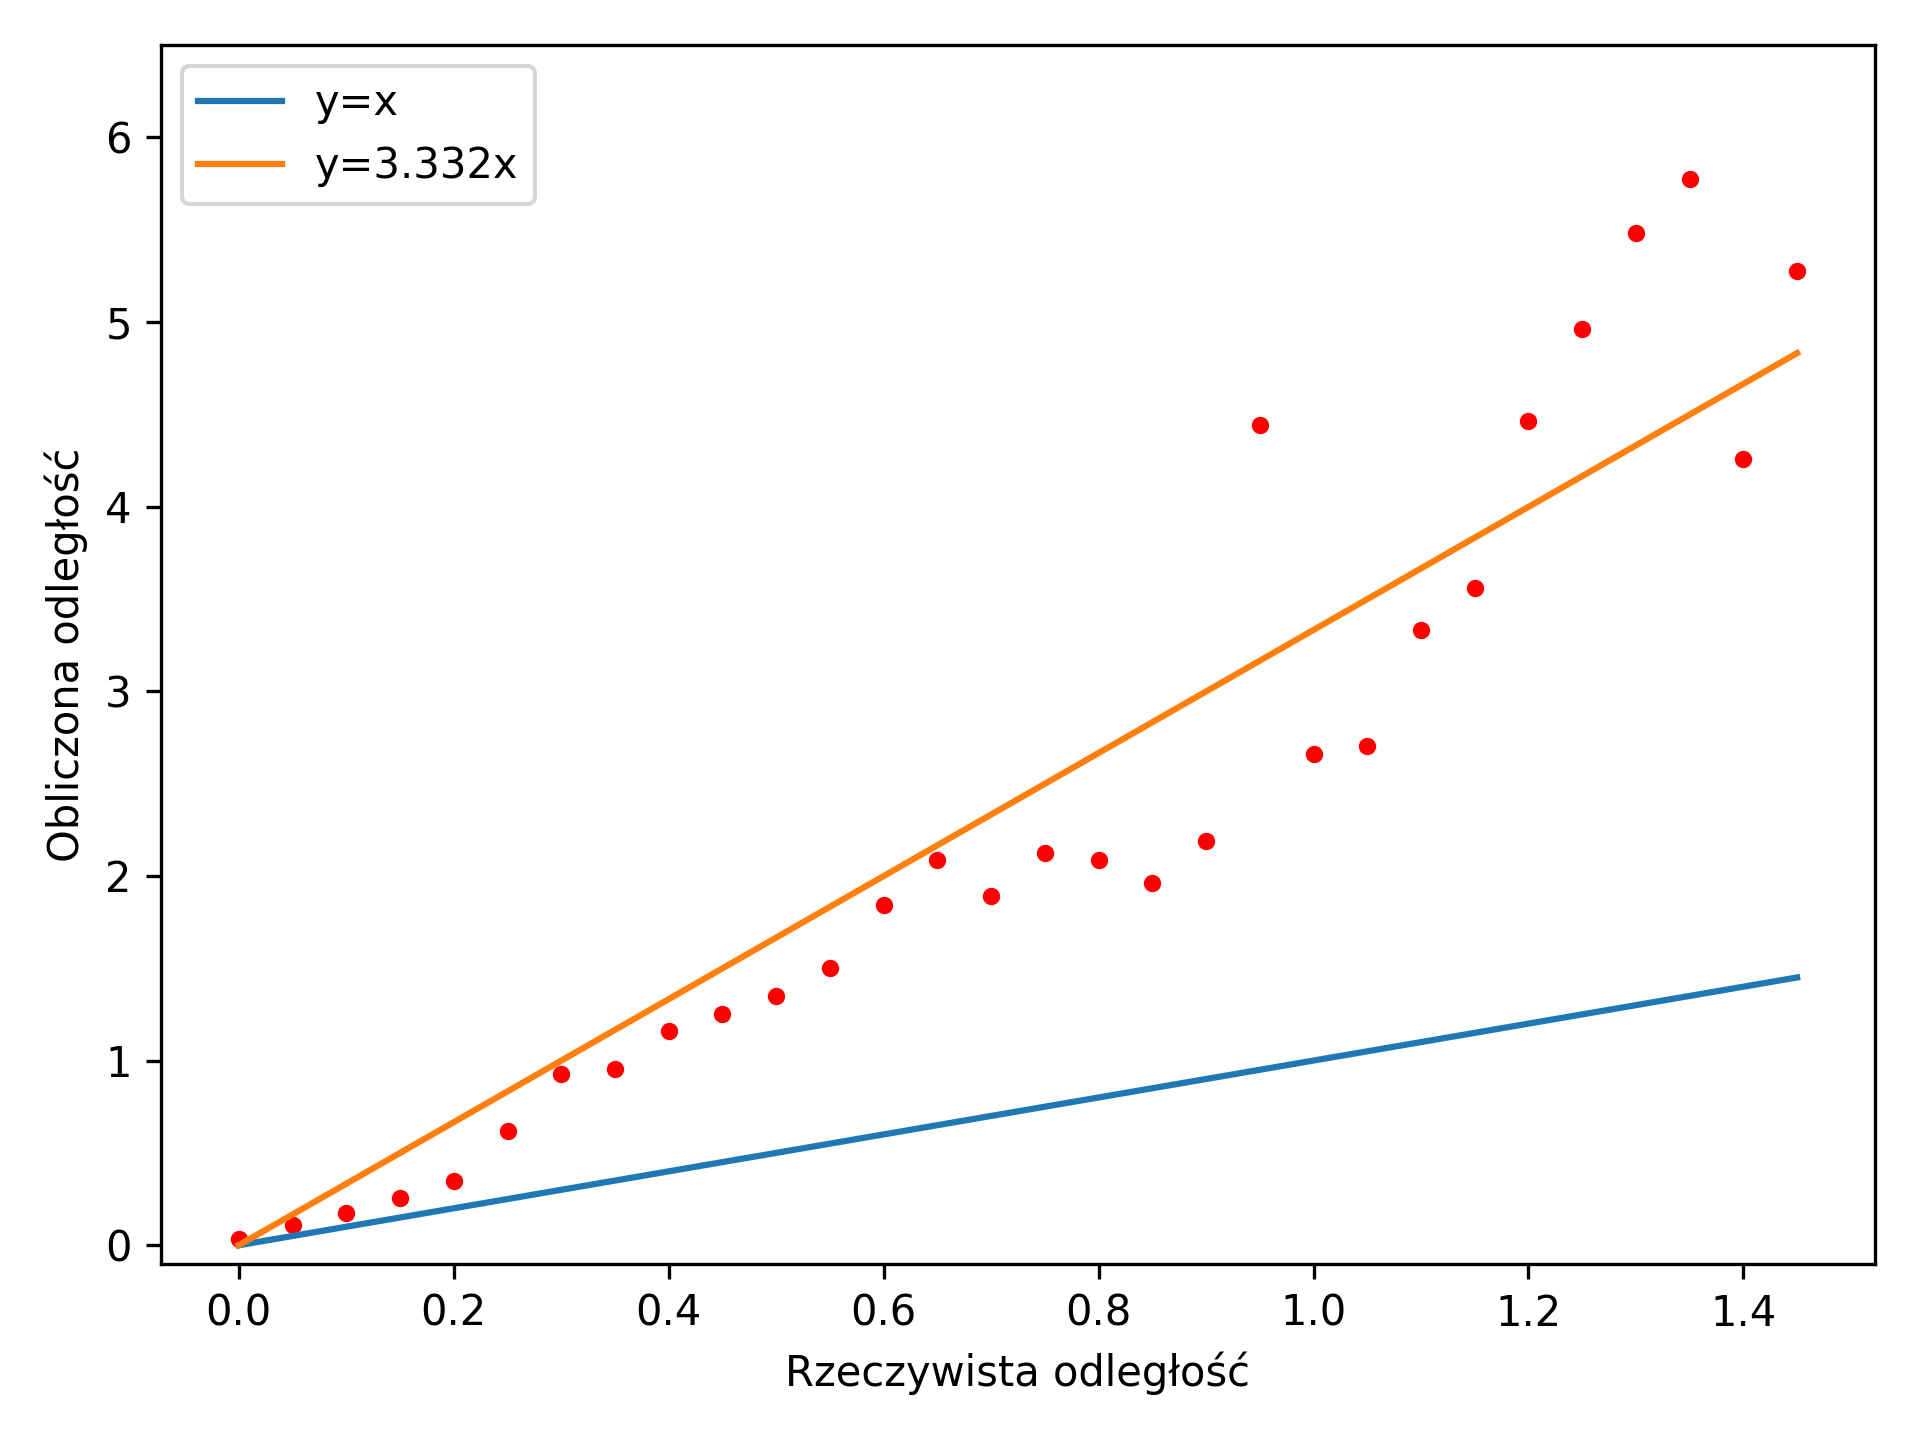
\includegraphics[width=.49\textwidth]{pics/mic_sync_dist/dists_close_long_3_mean.png}
\caption{Średnie obliczonych odległości}
\label{pic:slope_test_mean}
\end{figure}

Na wykresach można zauważyć trendy związane ze zmniejszającą się czułością wzmacniacza mikrofonu:

\begin{itemize}
    \item zmniejszanie się odległości punktu, w którym czułość jest zbyt mała by niezawodnie wyrywać nadawane sygnały,
    \item współczynnik prostej aproksymującej skalowane odległości rośnie.
\end{itemize}

Podobne efekty zaobserwowano kiedy brzęczyk nie był kierowany bezpośrednio w kierunku odbiornika.



\section{Ewaluacja działania systemu}

\begin{figure}[h]
\centering
    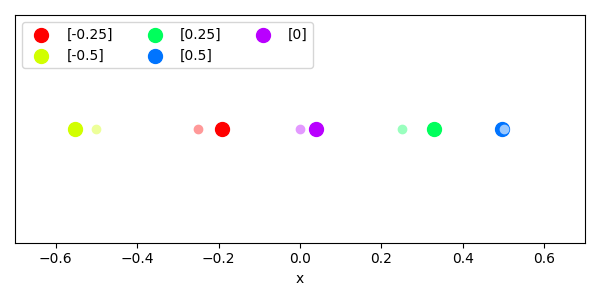
\includegraphics[width=.49\textwidth]{pics/mult_lat_1d/positions_2_mean.png}
    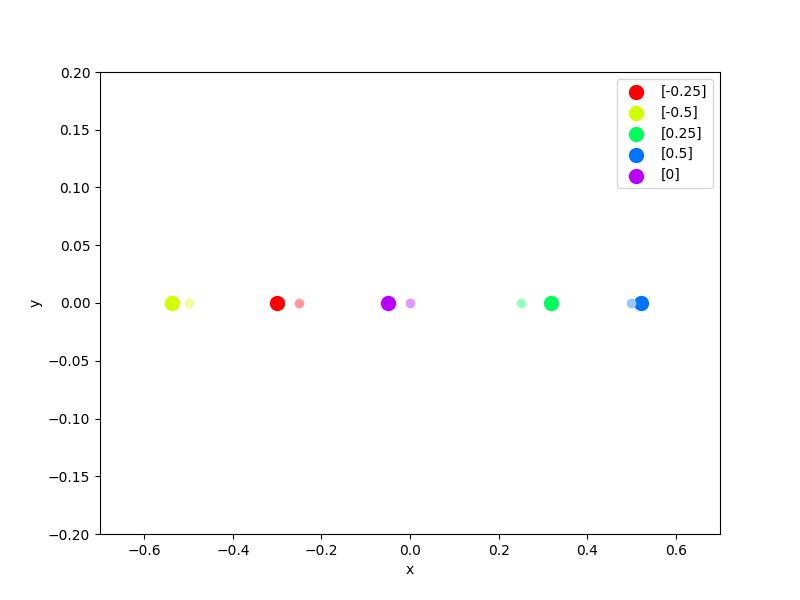
\includegraphics[width=.49\textwidth]{pics/mult_lat_1d/positions_4_mean.png}
\caption{Średnie obliczonych odległości}
% \label{pic:slope_test_mean}
\end{figure}

\begin{figure}[h]
\centering
    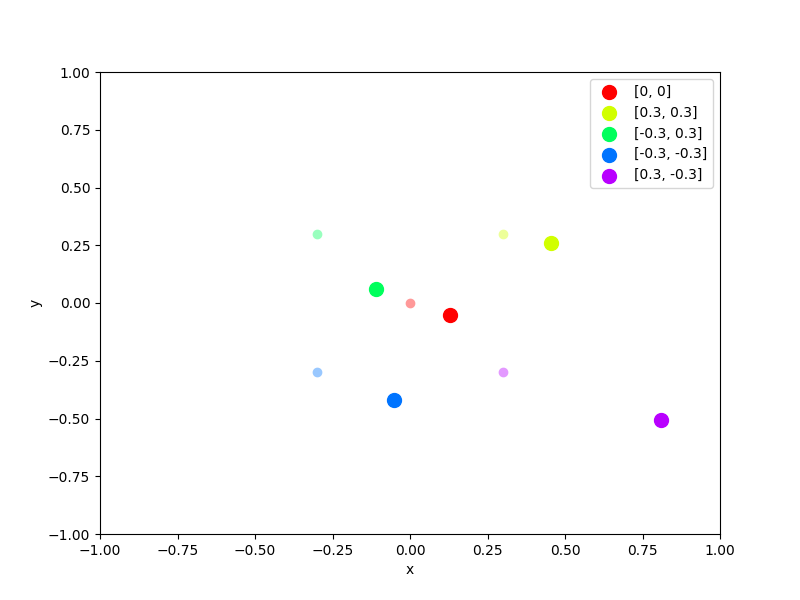
\includegraphics[width=.49\textwidth]{pics/mult_lat_2d/positions_1_mean.png}
    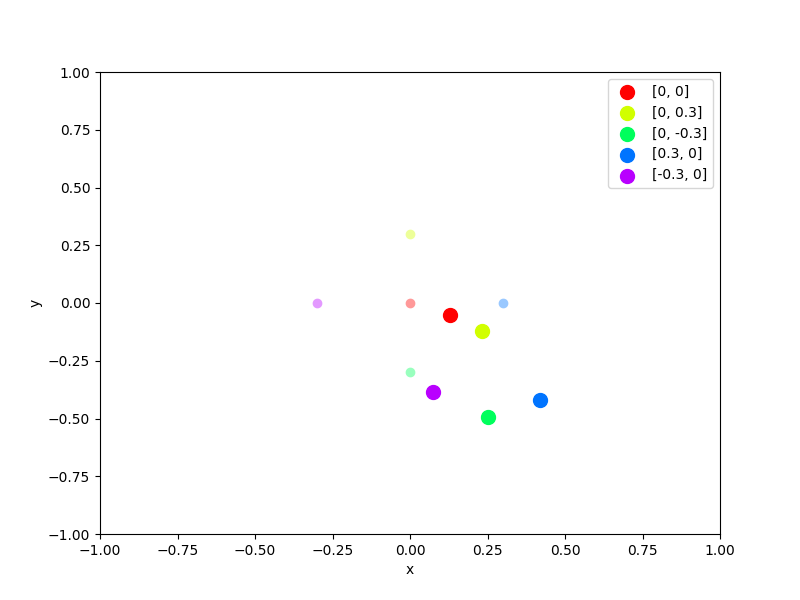
\includegraphics[width=.49\textwidth]{pics/mult_lat_2d/positions_2_mean.png}
    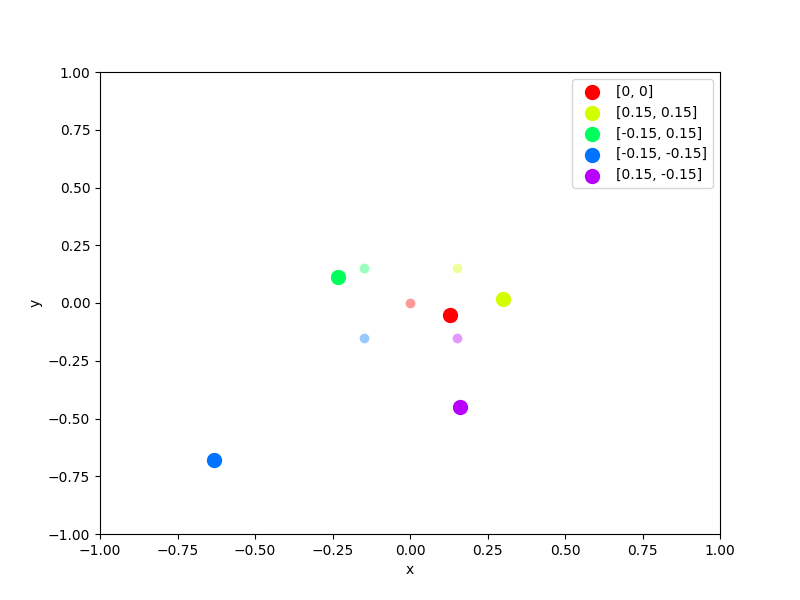
\includegraphics[width=.49\textwidth]{pics/mult_lat_2d/positions_3_mean.png}
\caption{Średnie obliczonych odległości}
% \label{pic:slope_test_mean}
\end{figure}

\begin{figure}[h]
\centering
    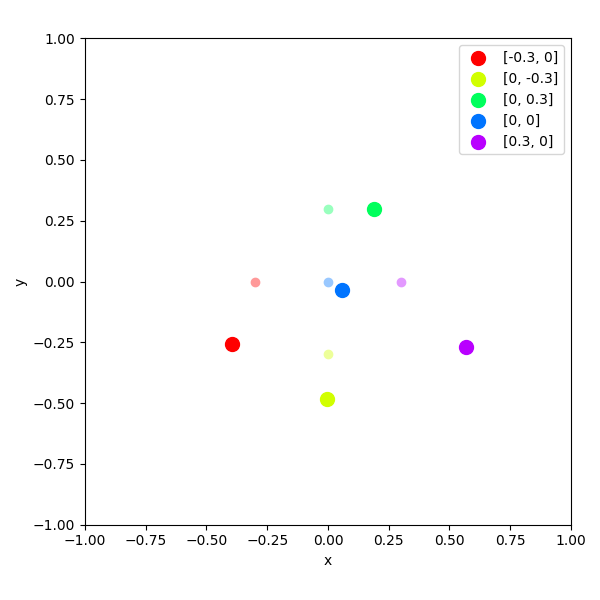
\includegraphics[width=.49\textwidth]{pics/mult_lat_2d_angle/positions_0_mean.png}
    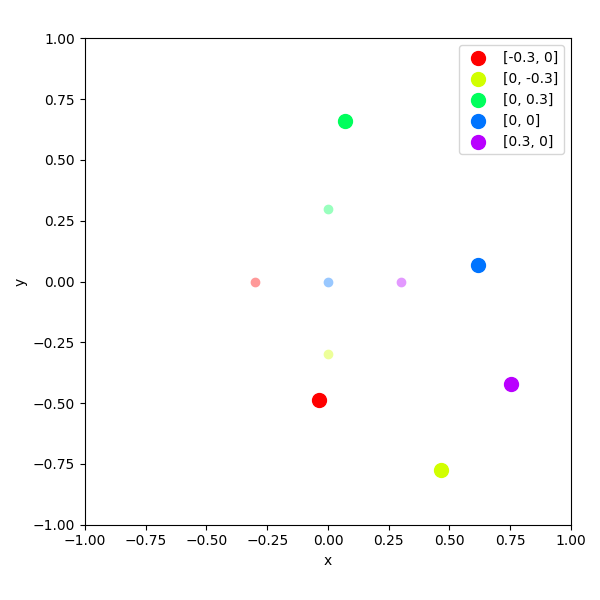
\includegraphics[width=.49\textwidth]{pics/mult_lat_2d_angle/positions_45_mean.png}
    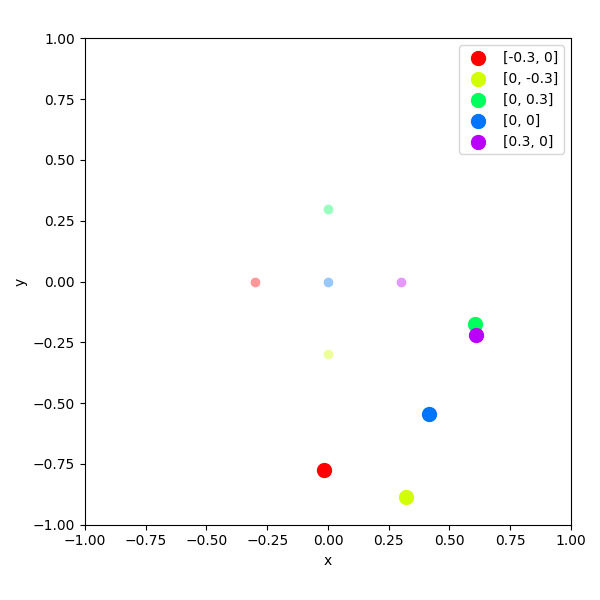
\includegraphics[width=.49\textwidth]{pics/mult_lat_2d_angle/positions_90_mean.png}
\caption{Średnie obliczonych odległości}
% \label{pic:slope_test_mean}
\end{figure}

\begin{figure}[h]
\centering
    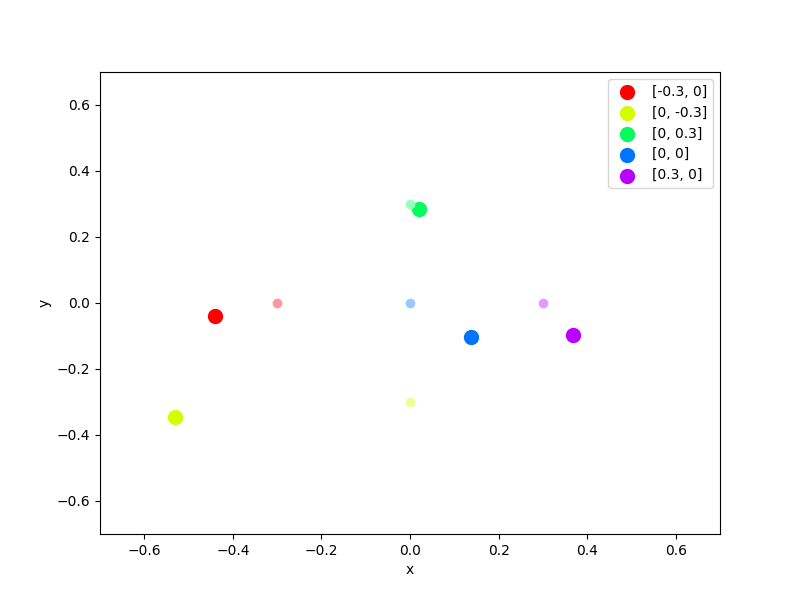
\includegraphics[width=.49\textwidth]{pics/mult_lat_2d_num/positions_3_mean.png}
    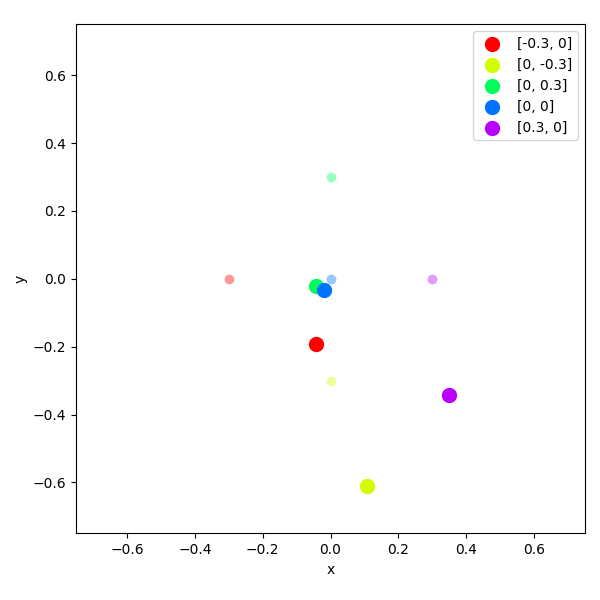
\includegraphics[width=.49\textwidth]{pics/mult_lat_2d_num/positions_4_mean.png}
    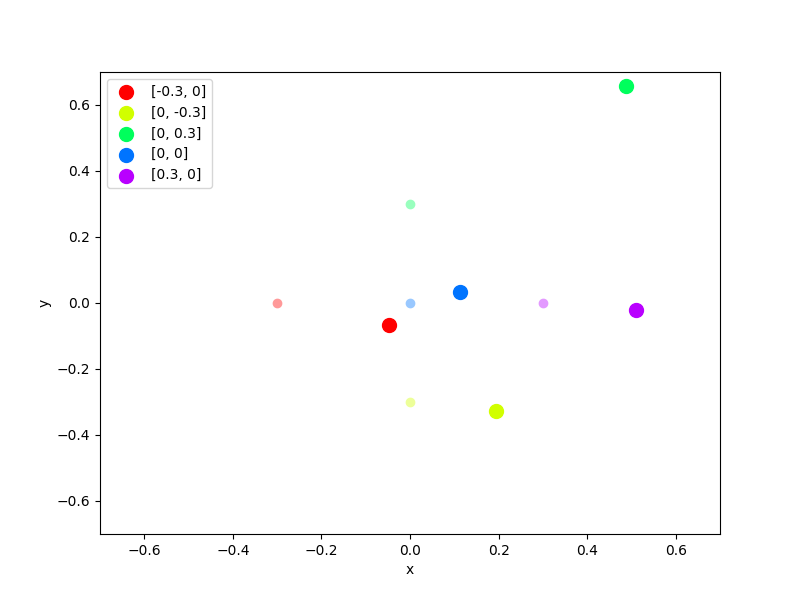
\includegraphics[width=.49\textwidth]{pics/mult_lat_2d_num/positions_5_mean.png}
    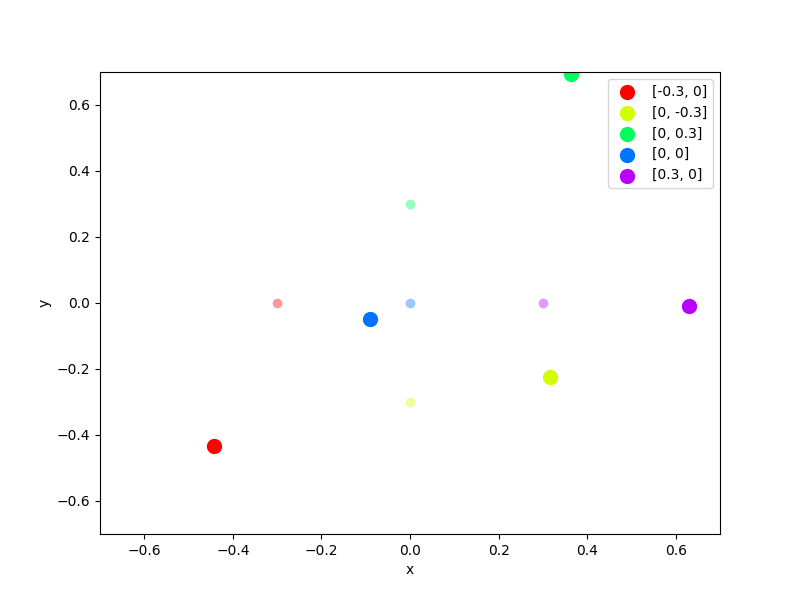
\includegraphics[width=.49\textwidth]{pics/mult_lat_2d_num/positions_6_mean.png}
    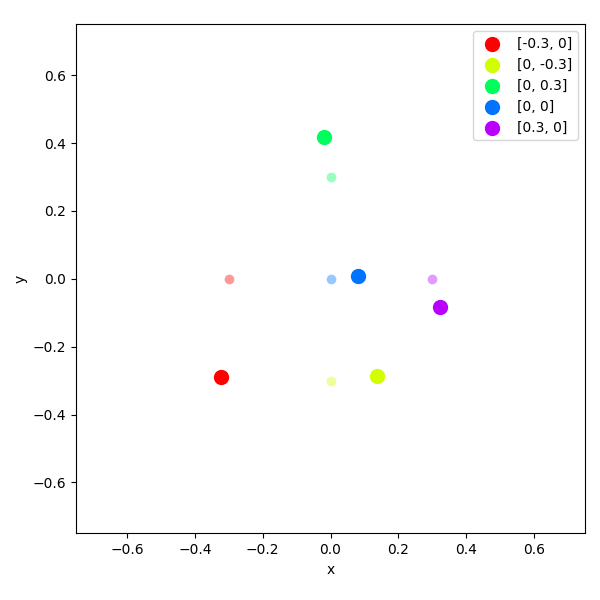
\includegraphics[width=.49\textwidth]{pics/mult_lat_2d_num/positions_7_mean.png}
    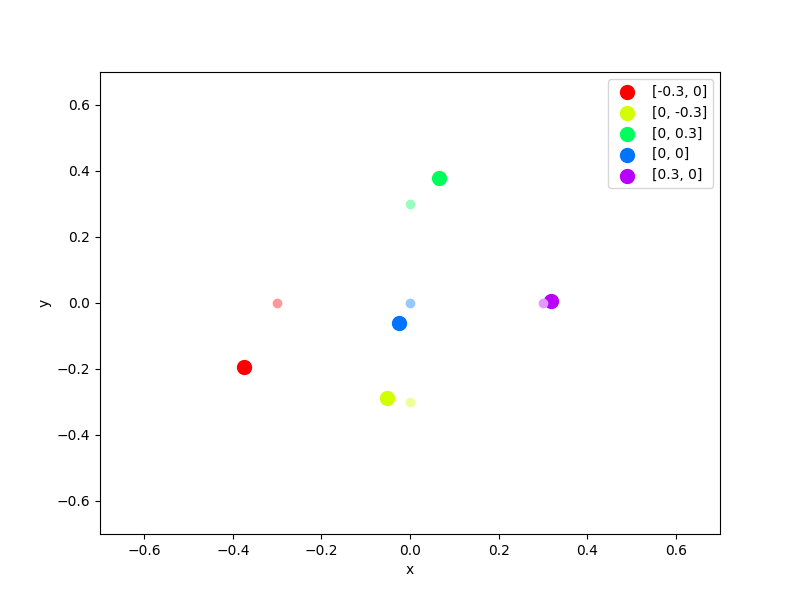
\includegraphics[width=.49\textwidth]{pics/mult_lat_2d_num/positions_8_mean.png}
\caption{Średnie obliczonych odległości}
% \label{pic:slope_test_mean}
\end{figure}

\section{Wyniki}

\subsection{Interpretacja}

\subsection{Wnioski}